\chapter{Methods}

\minitoc

\section{Curating a Benchmarking Dataset}

To establish a common ground for evaluating the performance of machine learning models, I curated a benchmarking dataset using data from various literatures. The main data source is the 2024 study by Mathis et al. which has the most diverse editing types ranging from 1-to-5bp replacement to 1-to-15bp deletions and insertions\cite{mathisMachineLearningPrediction2024}. It is complimented by the DeepPrime dataset, as it has a much bigger HEK293T dataset ($\sim290,000$ vs $\sim22,000$) as well as a wider range of cell type and PE pairs that can be used for fine-tuning the model to achieve better coverage and higher impact\cite{yuPredictionEfficienciesDiverse2023}. The mutated sequences in the datasets were masked by 'x', exposing only the region corresponding to PBS-RTT. To match the PRIDICT format, the mutated sequences were unmasked, and the missing regions due to the shorter wide sequence window is padded by `N'.


The dataset was parsed to preserve all essential information required by the models while also limiting the number of fields for better readability. More importantly, the standardized format allows easier conversion between datasets, with each data source requiring only two functions to allow universal usability, one to convert to and one to convert from standard format. The standard (std) format contains the following information:

\begin{itemize}[itemsep=-0mm]
    \item \textcolor{blue}{cell-line}: the cell line used in the experiment
    \item \textcolor{blue}{group-id}: the id of the target loci, used for grouping the data during cross validation
    \item \textcolor{blue}{mut-type}: the type of mutation introduced by the prime editor, 0 for replacements, 1 for insertions, 2 for deletions
    \item \textcolor{blue}{wt-sequence}: the 100bp/74bp long wild type target sequence starting from 10bp/4bp upstream of the protospacer(PRIDCT/DeepPrime dataset)
    \item \textcolor{blue}{mut-sequence}: the 100bp/74bp long edited target sequence starting from 4bp upstream of the protospacer(PRIDCT/DeepPrime dataset)
    \item \textcolor{blue}{protospacer-location}: the location of protospacer sequence complementary to sgRNA in the wild-type sequence 
    \item \textcolor{blue}{pbs-location}: the prime binding site
    \item \textcolor{blue}{rtt-location-wt/rtt-location-mut}: the location of reverse transcription template in the wild-type/edited sequence
    \item \textcolor{blue}{lha-location}: the location of left homology arm
    \item \textcolor{blue}{rha-location-wt/rha-location-mut}: the location of right homology arm in the wild-type/edited sequence
    \item \textcolor{blue}{spcas9-score}: precalculated SpCas9 score
    \item \textcolor{blue}{editing-result}: empirically observed editing efficiency
\end{itemize}

The locations are separated into two columns in the format of "start:end", where start is the 0-based index of the first base of the sequence, while end is for last base of the sequence(non-inclusive). All sequences were read in the direction of from protospacer to PAM for easier interpretation. This is often different from previous studies that read from 5' end to the 3' end of the pegRNA instead of using their relative position to the target sequence.

The data files are named as ``\{format\}-\{source\}-\{cell-line\}-\{PE-version\}.csv". `format' can be `std' for standard format, `shap' for files with only extracted features, as well as formats for individual models containing all the data required for training, such as `pd' for PRIDICT and `dp' for DeepPrime. `source' is the name of the study that the data was extracted from, while `cell-line' and `PE-version' are self explanatory.

Five main datasets of size greater than 10,000 were used frequently for benchmarking in this study: DeepPrime HEK293T PE2, PRIDICT2.0 HEK293T, PRIDICT2.0 K562, PRIDICT2.0 K562MLH1d, and PRIDICT2.0 Adv. The HEK293T cells refer to the human embryonic kidney cells\cite{kavsanImmortalizedCellsOne2011}; `Adv' refers to prime editing performed in-vivo (in a living organism) in mouse liver cells; K562 cells were derived from a chronic myelogenous leukemia patient\cite{lozzioMultipotentialLeukemiaCell1981} (K562MLH1d refers to K562 cells with MMR inhibition using the MLH1dn proteins). Other smaller datasets were used for fine tuning models trained with the DeepPrime HEK293T PE2 dataset, such as the DeepPrime HEK293T PE2-Max dataset.

The editing efficiencies were calculated using the method suggested by Kim et al.\cite{kimPredictingEfficiencyPrime2021} in \autoref{eq:efficiency}, which was also used by PRIDICT:
\begin{equation}
    \label{eq:efficiency}
    \begin{split}
        \text{Editing Efficiency} =& \frac{\text{Edited Count}}{\text{Total Count}} \times 100\% \\
    \end{split}
\end{equation}
Where:
\begin{equation}
    \begin{split}
        \text{Edited Count} =& \text{Read Counts With Intended Edit at Target Site} - \\
        &( \text{Total Read Counts} \times \text{Background Editing  Rate} ) \\
        \text{Total Count} =& \text{Total Read Counts} - (\text{Total Read Counts} \times \\ &\text{Background Editing  Rate})
    \end{split}
\end{equation}
        
Background editing rate refers to the percentage of target loci that were edited without being transfected with the prime editor. Subtracting the background edits from the total read counts gives the estimated true number of reads that were edited by the prime editor.

The datasets are split into 5 folds based on the group id assigned to each target loci and pegRNA combination. Edits on the same target loci have the same group id, and are thus placed in the same fold to prevent data leakage. The folds are then used for cross validation to evaluate the model's performance.



\section{Data Engineering}
\label{sec:data-engineering}

A conspicuous issue with the dataset is the imbalance in target values. Shown in Figure \ref{fig:imbalanced-original}, the distribution of the editing efficiency is heavily skewed towards the lower end, with a large number of pegRNAs having an efficiency of around 0. This can cause the model to be less accurate in predicting the higher efficiency pegRNAs, as the model would be more inclined to predict lower efficiency to minimize the loss. 

\begin{figure}
    \centering
    \subfigure[Original]{
        \label{fig:imbalanced-original}
        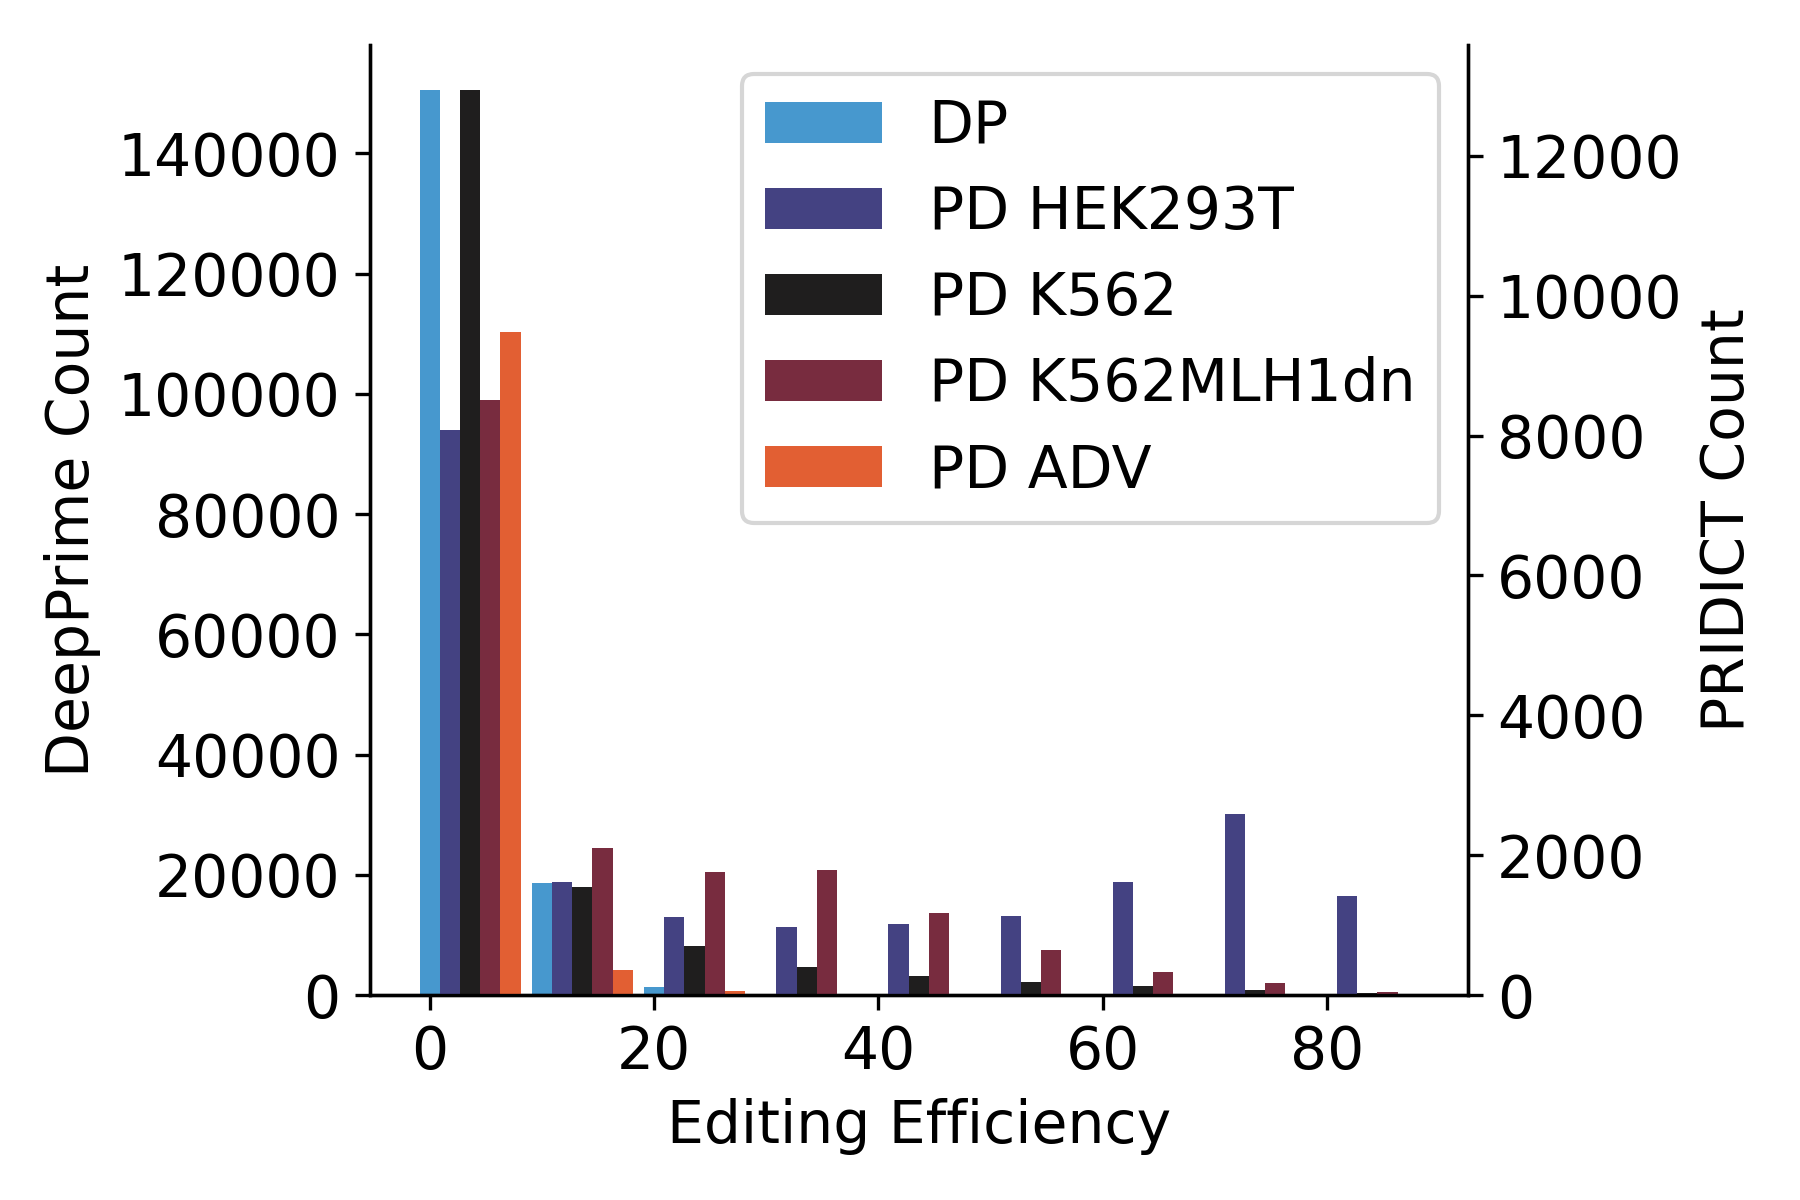
\includegraphics[width=0.45\textwidth]{editing-efficiency-comparison.png}
    }
    \subfigure[Log Adjusted]{
        \label{fig:imbalanced-log}
        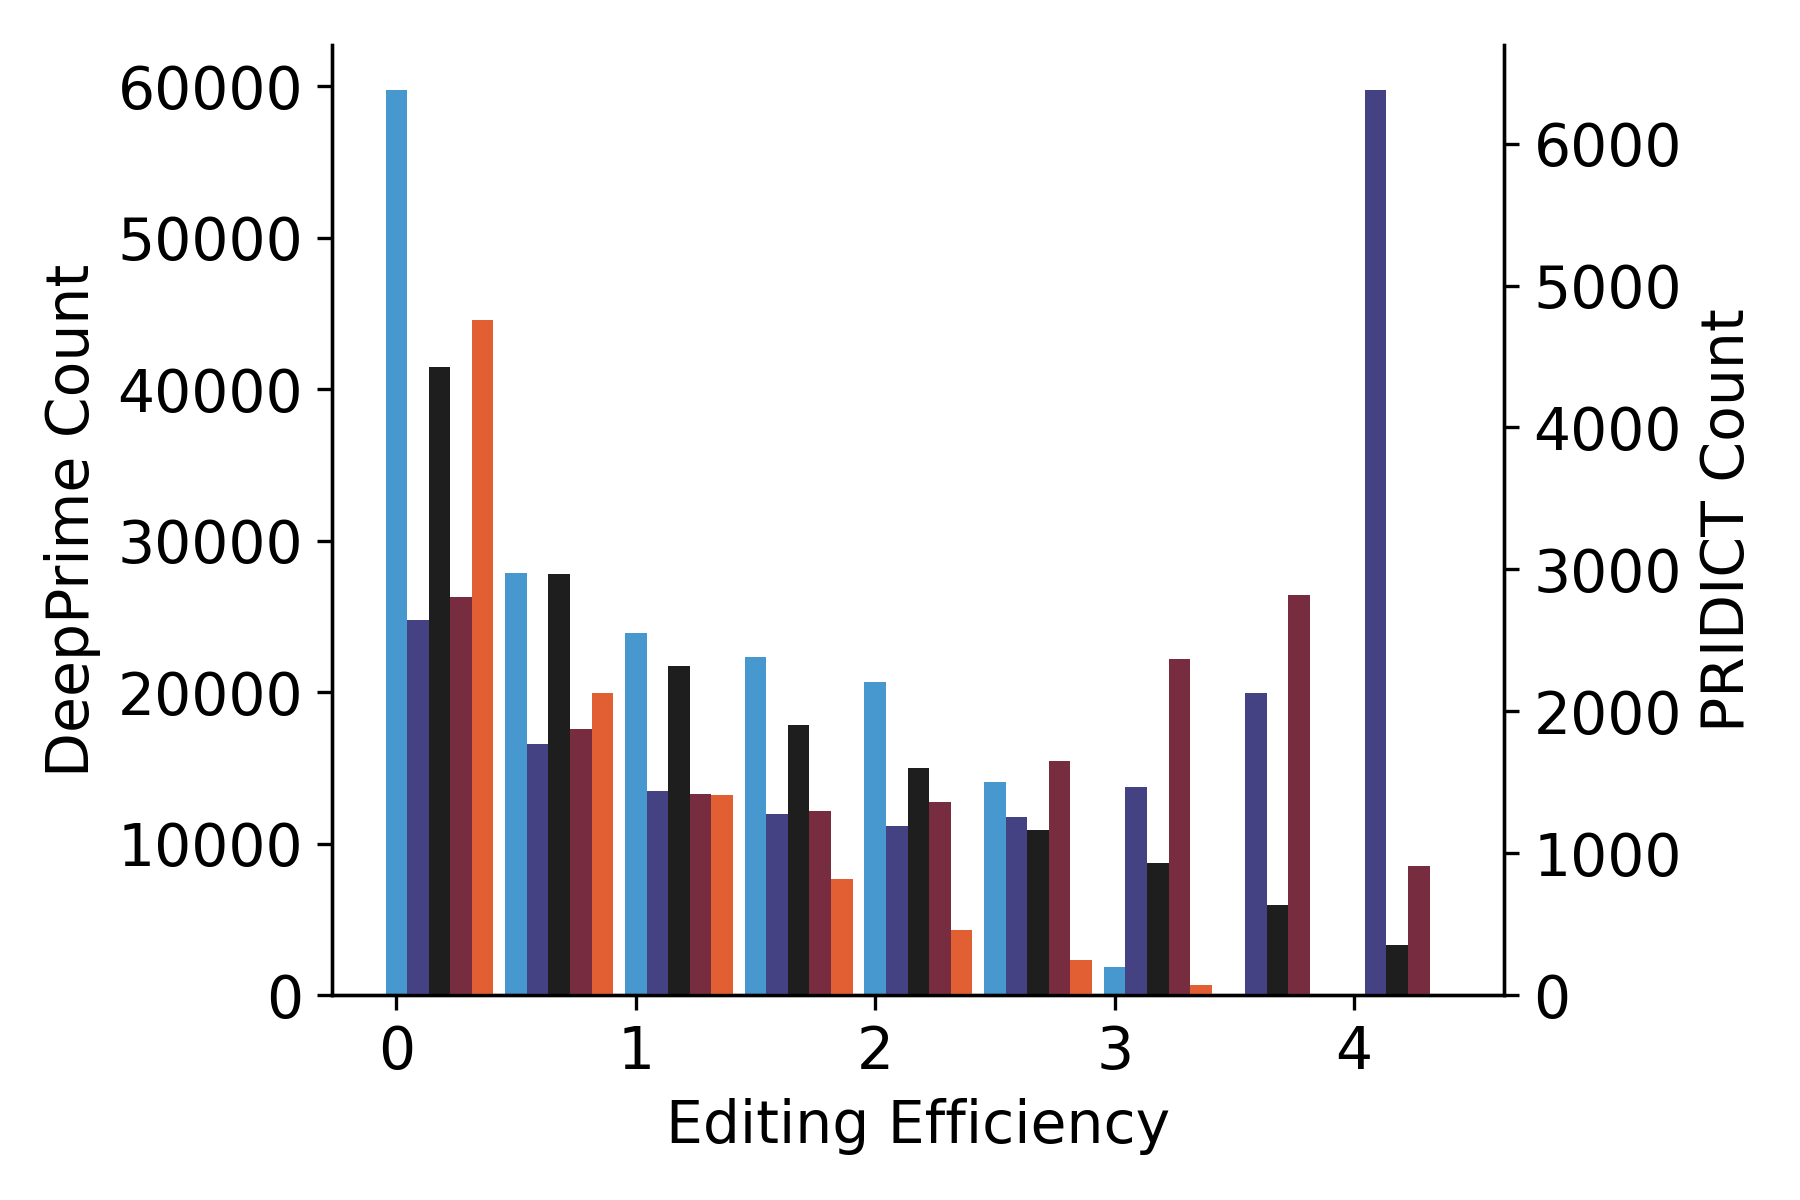
\includegraphics[width=0.45\textwidth]{editing-efficiency-log-adjusted.png}
    }
    \subfigure[Undersampling]{
        \label{fig:imbalanced-undersampling}
        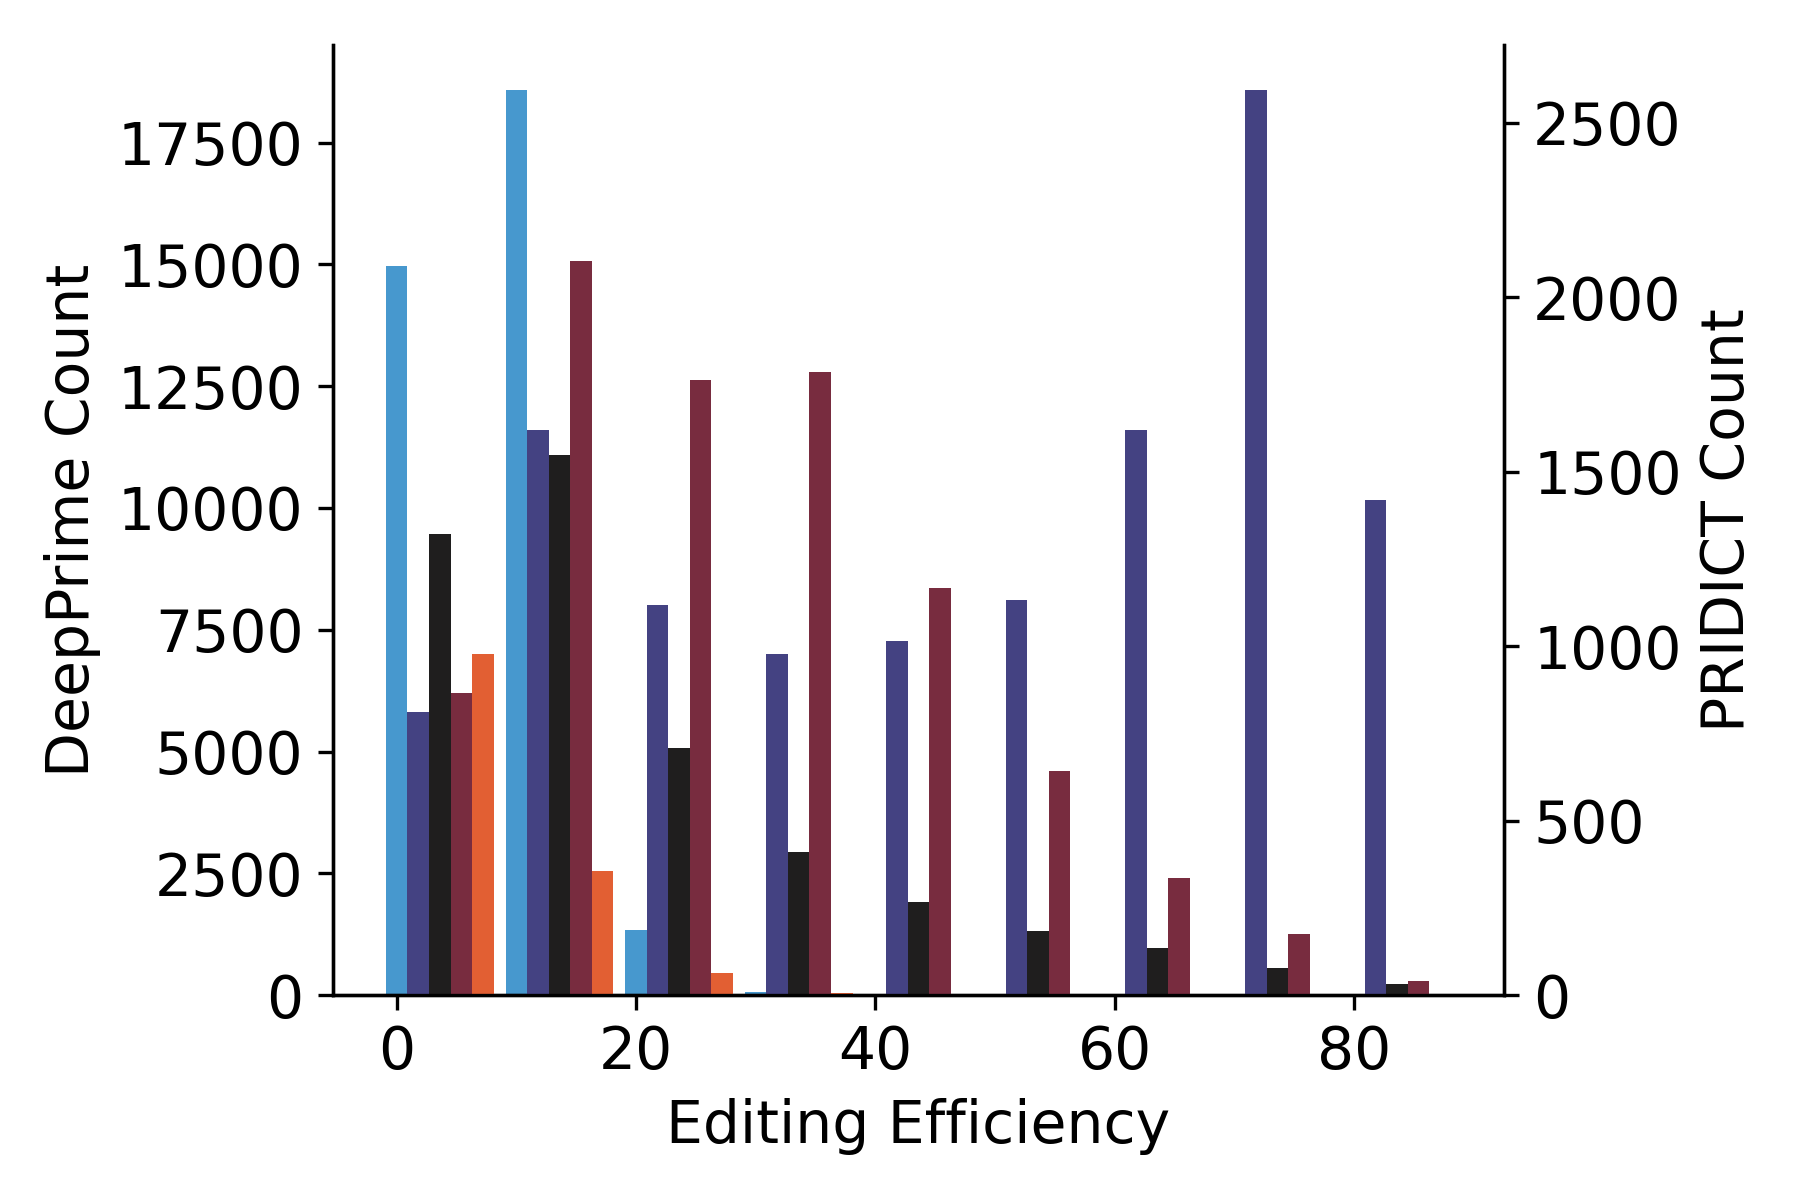
\includegraphics[width=0.45\textwidth]{editing-efficiency-undersample.png}
    }
    \subfigure[Quantile transformation]{
        \label{fig:imbalanced-quantile}
        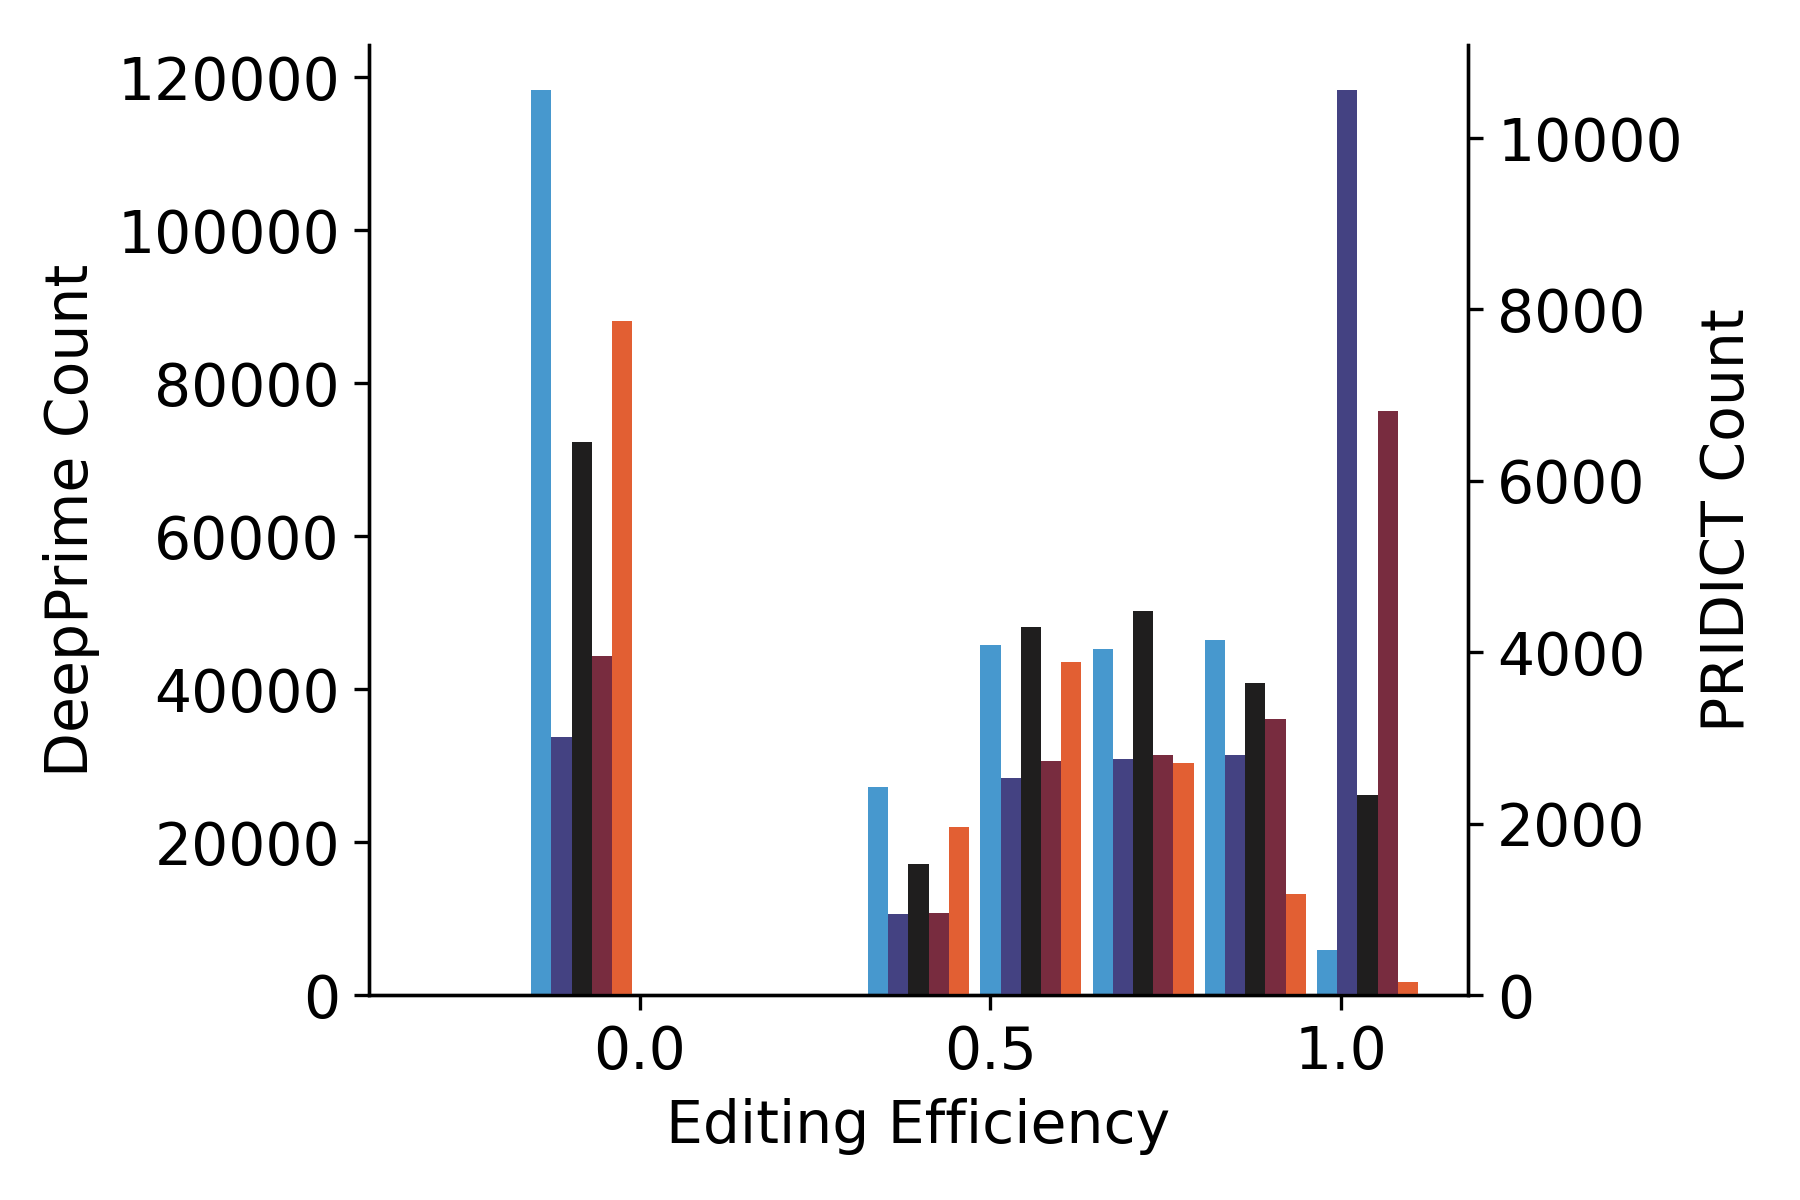
\includegraphics[width=0.45\textwidth]{editing-efficiency-quantile-transform.png}
    }
    \label{fig:imbalanced}
    \caption[Target Distribution Imbalance]{The distribution of the editing efficiency in the DeepPrime HEK293T PE2 (DP) dataset, the PRIDICT2.0 HEK293T (PD HEK293T) dataset, the PRIDICT2.0 K562 (PD K562) as well as K562 MMR deficient (PD K562MLH1DN) dataset, and the PRIDICT2.0 Adv (PD ADV) dataset. (a), followed by the distribution after several adjustments (b-d). Due to the significant different in dataset sizes, DeepPrime datasets and PRIDICT datasets used different y-axis scale (left and right for DeepPrime and PRIDICT respectively): 
    \textbf{(a)} the distribution of original editing efficiency in the datasets. editing efficiency on the x axis is limited to [0, 100], with bin size of 10; \textbf{(b)} the distribution of the log adjusted editing efficiency in the DeepPrime HEK293T PE2 dataset; \textbf{(c)} the distribution of the editing efficiency after undersampling the data with editing efficiency $<10$ with a ratio of 10:1 (10\% of the original data were preserved); \textbf{(d)}, the distribution of the editing efficiency after uniformly quantile transformed.}
\end{figure}

Although the research for imbalanced regression task is relatively limited compared to classification, a number of methods have been proposed\cite{krawczykLearningImbalancedData2016}. The simplest method is to adjust the target values so that better balance can be achieved in the projected space. Log transformation is a suitable method for the editing efficiency dataset, as it increases the distance between the lower values while keeping the higher values close (Figure \ref{fig:imbalanced-log}). The numpy \verb|log1p| function was used to prevent the transformation from being undefined when the target value is 0. During inference, the predicted values were transformed back to the original scale using the \verb|expm1| function. Undersampling is also a useful technique, by removing the majority of the lower efficiency pegRNAs, the model can be trained to better predict the higher efficiency pegRNAs\cite{torgoResamplingStrategiesRegression2015}. 
The undersampling ratio was set to 10:1, with the majority of the pegRNAs with efficiency $<10$ removed (Figure \ref{fig:imbalanced-undersampling}). The undersampling ratio and threshold for determining the part of the data to undersample was fine tuned in the list of [20:1, 15:1, 10:1, 5:1] and [5, 10, 15] respectively using a XGBoost model trained on the first fold of DeepPrime HEK293T PE2 dataset. 
SMOTE (Synthetic Minority Over-sampling Technique) was also considered, but the generation of synthetic data is very difficult for the prime editing prediction task, as the pegRNA sequence is highly structured and the synthetic data generated may not be biologically feasible. Additionally, quantile transformation was also tested. However, since it discretizes the data, some precision is expected to be lost during the inverse transformation.

In addition to adjusting the dataset itself, the loss function can also be adjusted to assign different importance to different target values. Sample weights can be used to penalize the model more for mispredicting the higher efficiency pegRNAs. 


DeepPrime applied a weighted loss function of the editing efficiency tuned for their dataset:
\begin{equation}
    \text{weight} = \text{min}(\exp(6(\log(x+1)-3)+1),5)
\end{equation}
where x is the measured editing efficiency. The weight is then used in the loss function to penalize the model more for mispredicting the higher efficiency pegRNAs.

At the mean time, PRIDICT did not report any special treatment for the imbalanced dataset, possibly because the having high accuracy for the lower efficiency pegRNAs is as important as predicting the performance higher efficiency pegRNAs accurately. 

To verify if the adjustments had made any significant different on the model's performance, a simple two layer MLP with 128 hidden units in each layer was trained on the DeepPrime HEK293T PE2 dataset using the original, log adjusted, undersampled and quantile transformed datasets. An additional model using the DeepPrime adjusted MSE was also tested. The models were trained using the Adam optimizer with a learning rate of 0.005, and the learning rate was adjusted using the CosineAnnealingLRWarmRestart scheduler, with a T\_0 (epoch of the first restart) of 15 and T\_mult (the factor to extend the restart intervals) of 1 to escape local minima. 

\begin{figure}
    \centering
    \vspace{-3mm} % Reduce vertical space between subfigures
    \subfigure[DP HEK293T]{
        \centering
        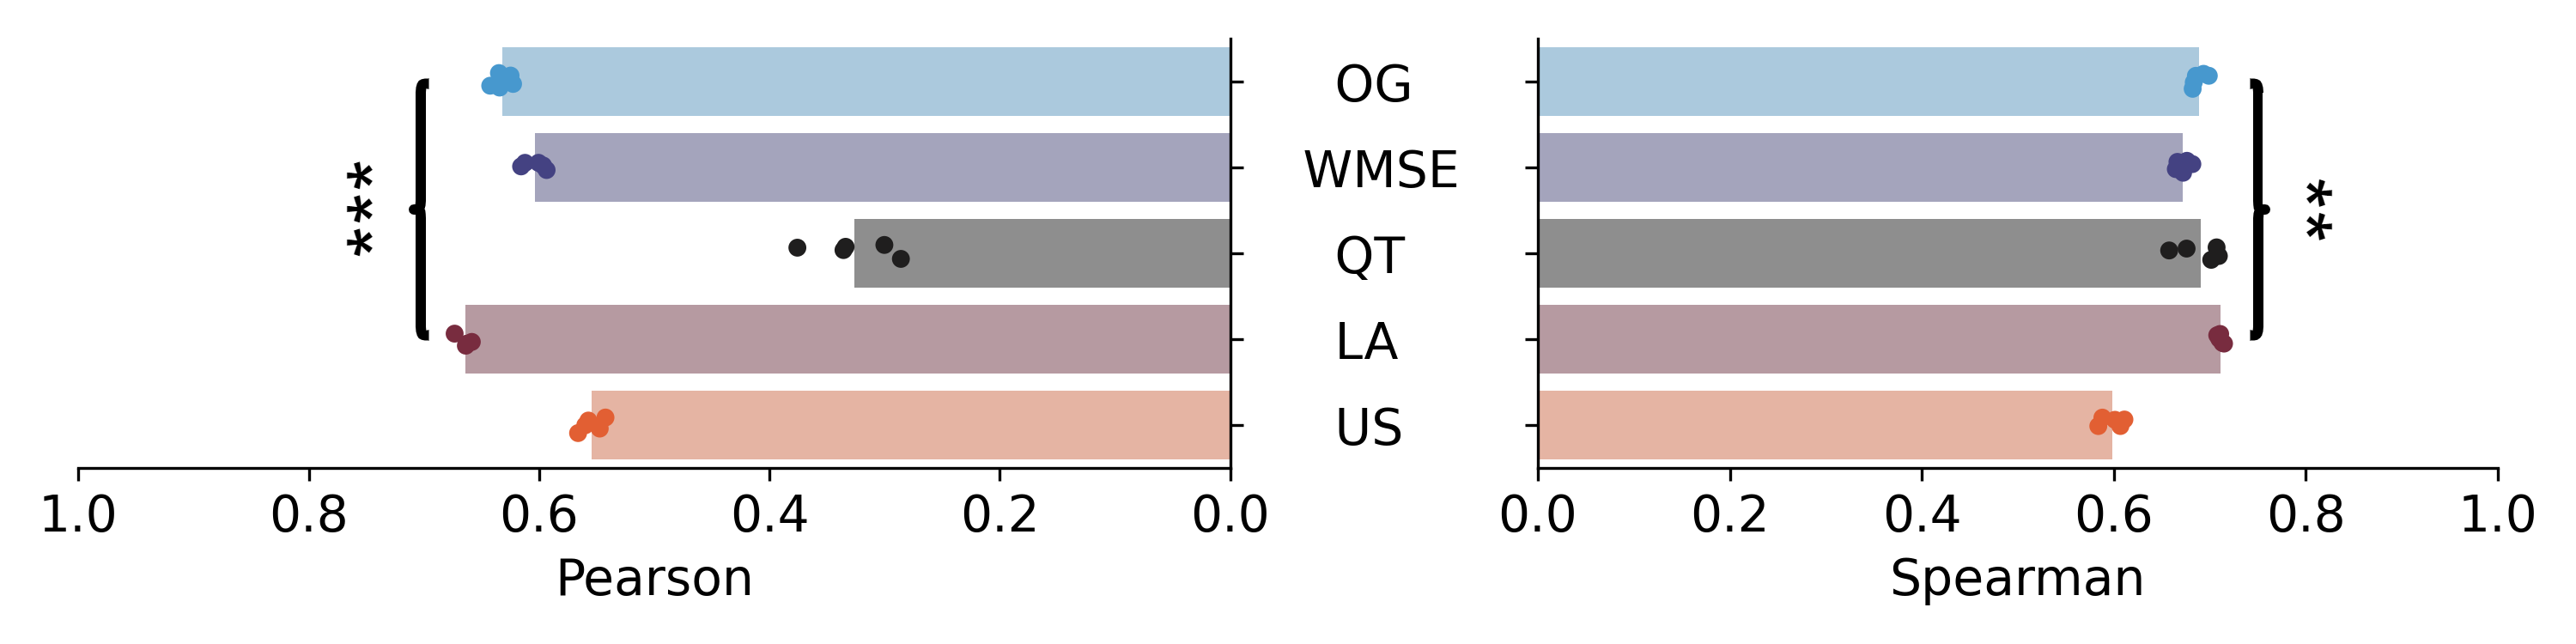
\includegraphics[width=0.8\textwidth]{adjustment-dp-hek293t-performance.png}
        \label{fig:dp-hek293t-adjustment-performance}
    }
    \vspace{-3mm}
    \subfigure[PD HEK293T]{
        \centering
        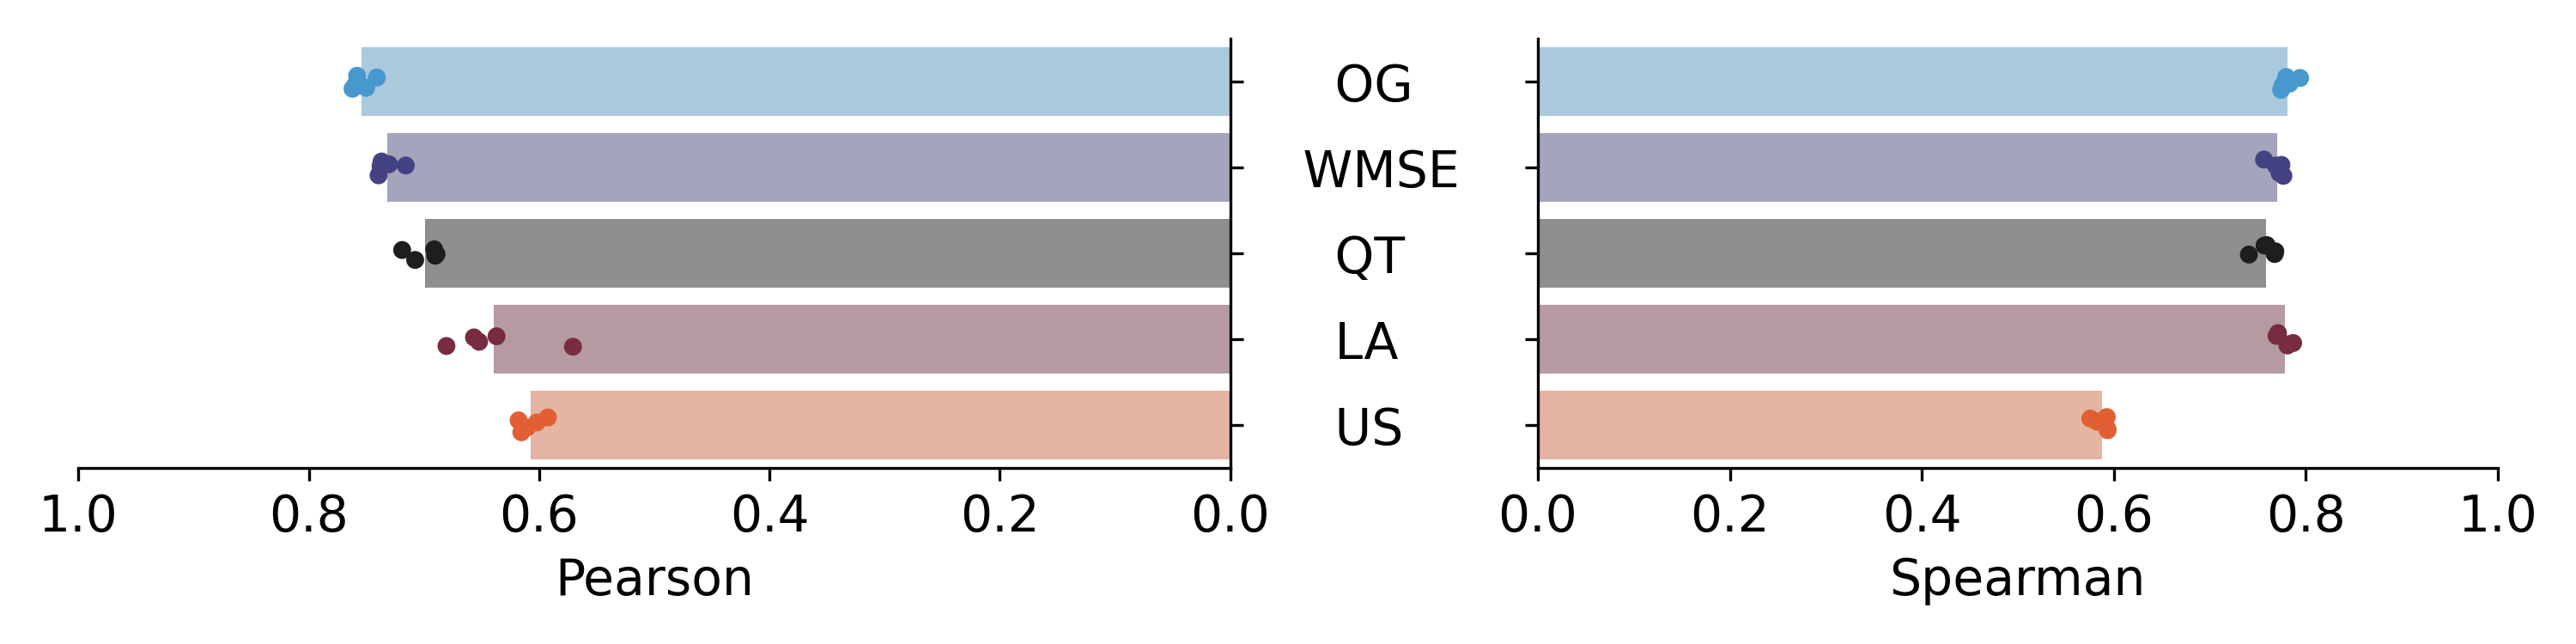
\includegraphics[width=0.8\textwidth]{adjustment-pd-hek293t-performance.png}
        \label{fig:pd-hek293t-adjustment-performance}
    }
    \vspace{-3mm}
    \subfigure[PD K562]{
        \centering
        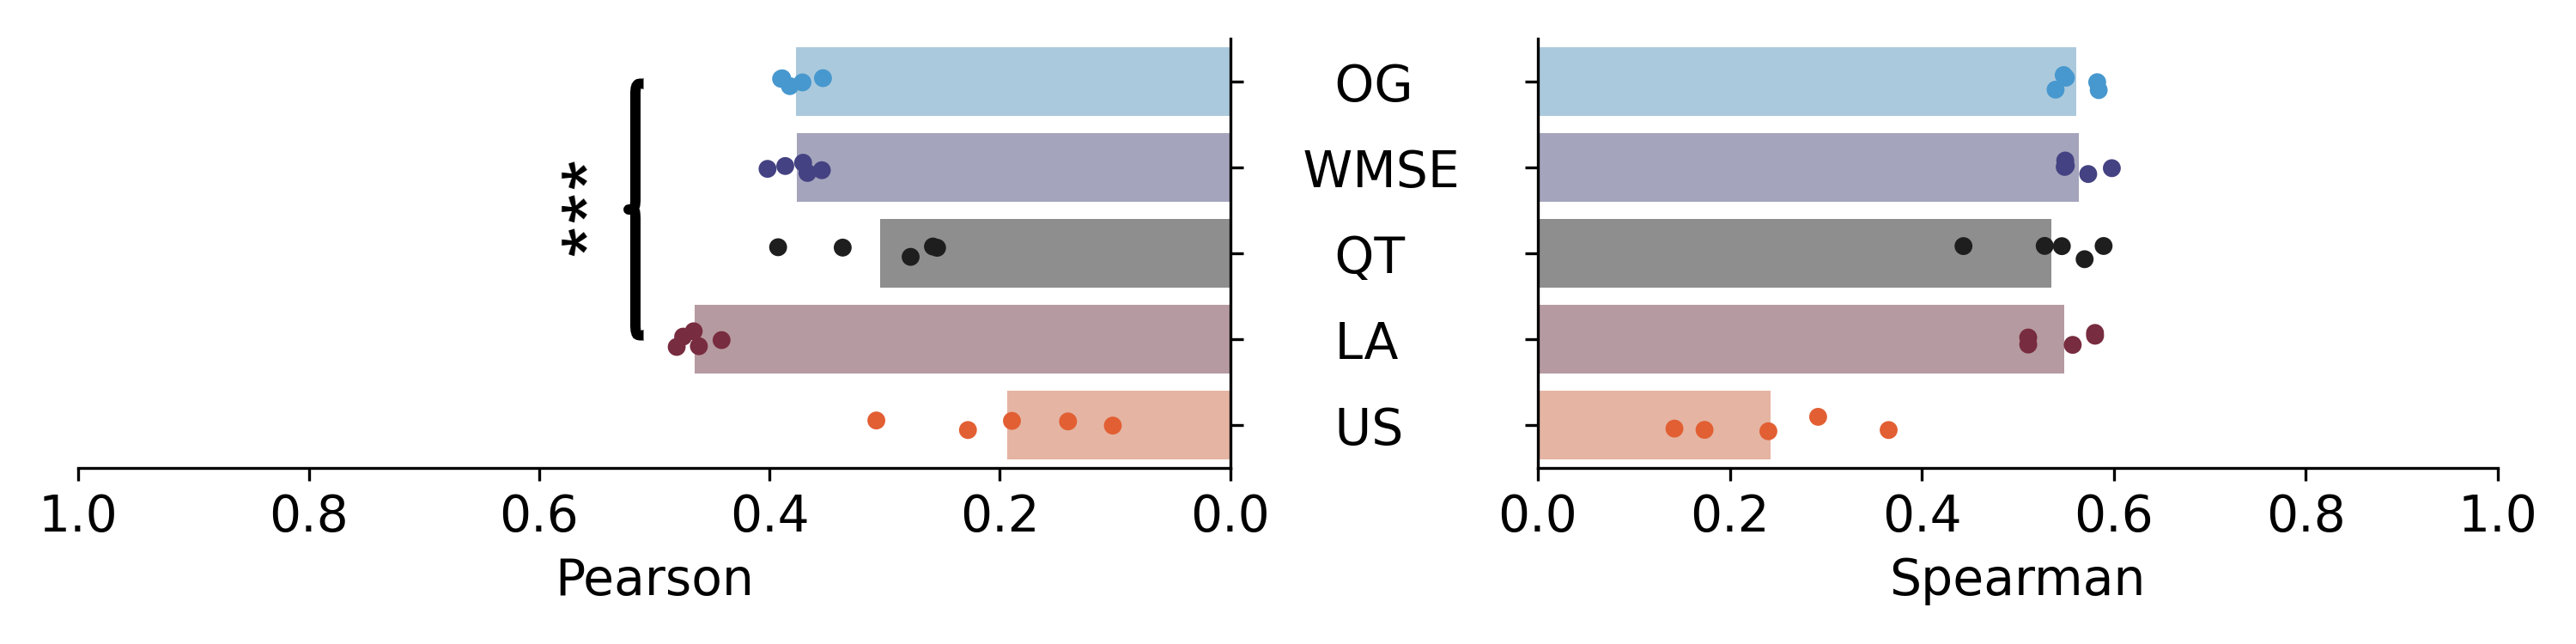
\includegraphics[width=0.8\textwidth]{adjustment-pd-k562-performance.png}
        \label{fig:pd-k562-adjustment-performance}
    }
    \vspace{-3mm}
    \subfigure[PD K562MLH1dn]{
        \centering
        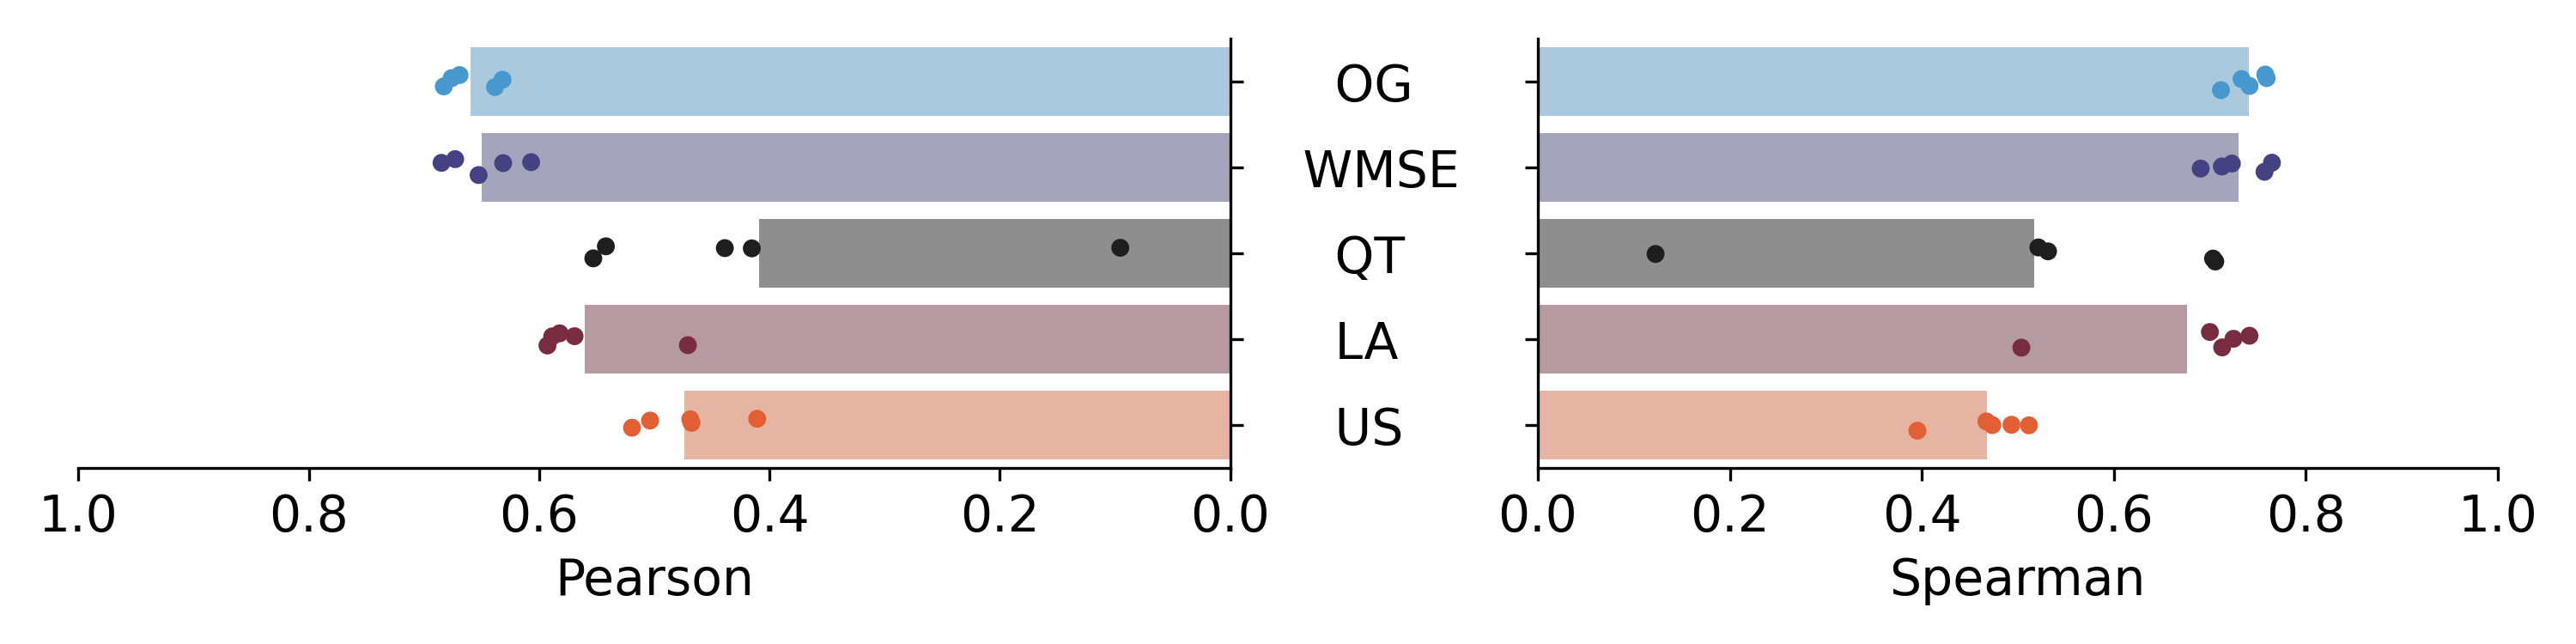
\includegraphics[width=0.8\textwidth]{adjustment-pd-k562mlh1d-performance.png}
        \label{fig:pd-k562mlh1d-adjustment-performance}
    }
    \vspace{-3mm}
    \subfigure[PD Adv]{
        \centering
        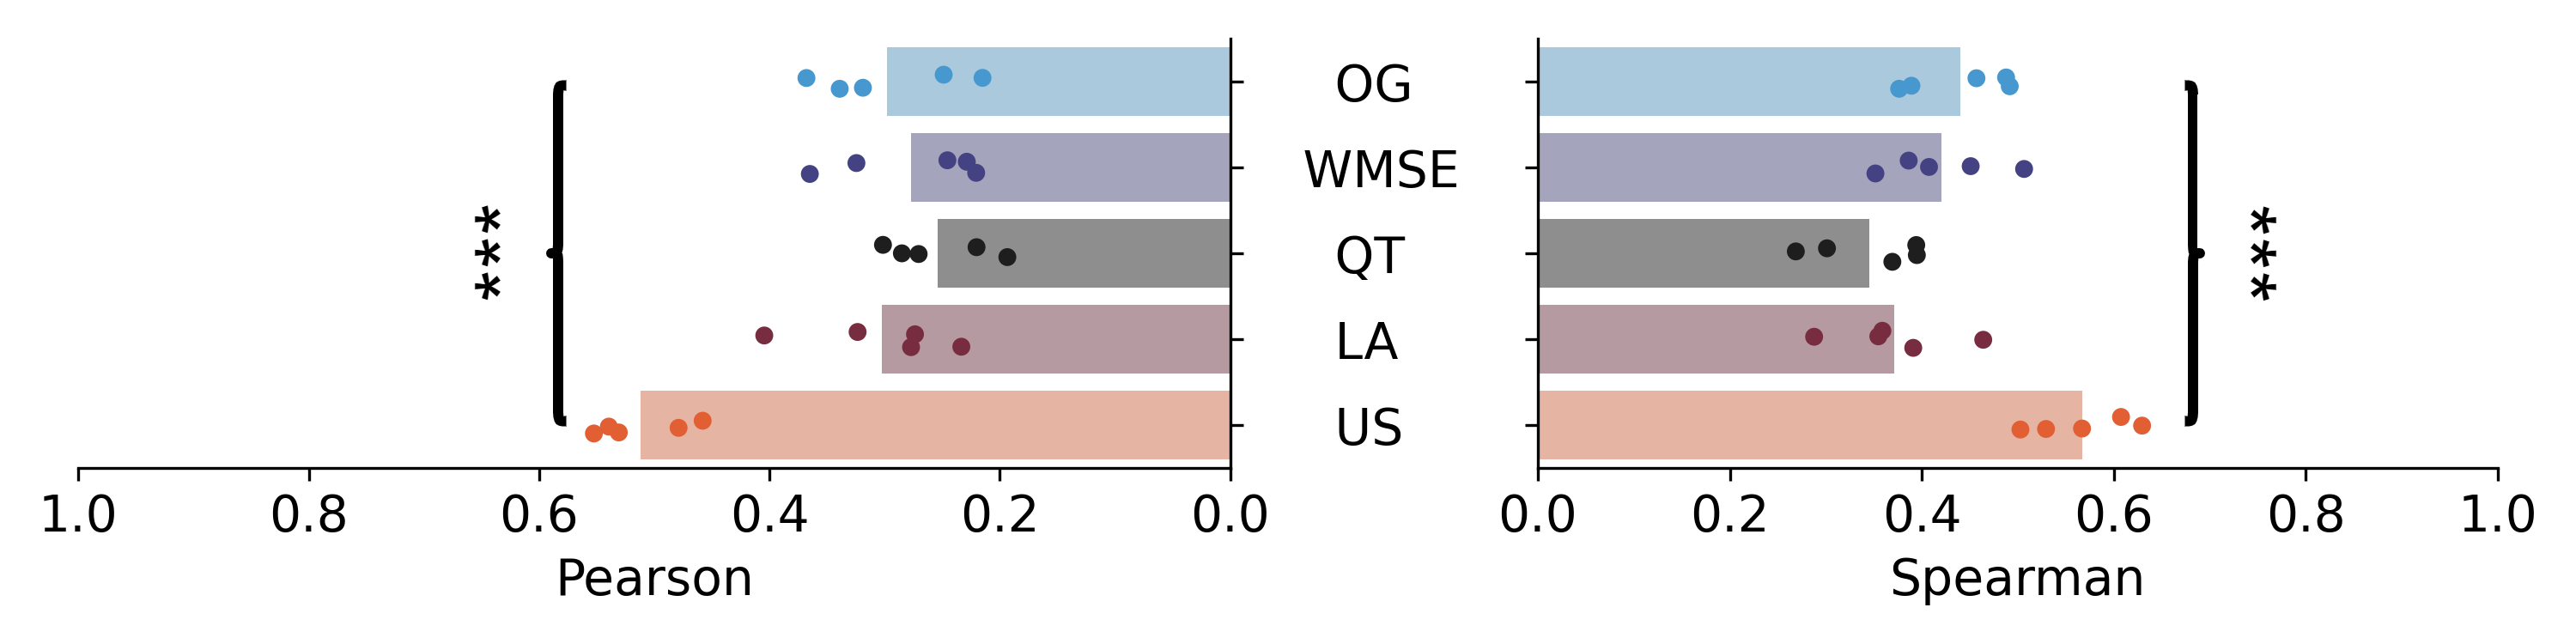
\includegraphics[width=0.8\textwidth]{adjustment-pd-adv-performance.png}
        \label{fig:pd-adv-adjustment-performance}
    }
    \caption[DeepPrime model performance comparison after adjustments]{Performance comparison of the DeepPrime model trained on the DeepPrime HEK293T PE2 dataset. The asterisks indicating significance are only shown when an adjustment performed significantly \textbf{better} than training on original data. \textbf{(a)}, the PRIDICT2.0 HEK293T dataset \textbf{(b)}, the PRIDICT2.0 K562 dataset (PD K562\textbf{(c)}), the PRIDICT2.0 K562MLH1d dataset \textbf{(d)}, and the PRIDICT2.0 Adv dataset \textbf{(e)} using the log adjusted (LA), undersampled (US), quantile transformed (QT), and DeepPrime weighted MSE (WMSE) adjustments, in addition to the original dataset and citerion (OG). 
    The performance of each fold is shown as a strip plot on top of the matching bar.}
    \label{fig:adjustment-performance}
\end{figure}

The result of the five adjustments on the five datasets are shown in \autoref{fig:adjustment-performance}. Significant improvements were only observed in three occasions ($p<0.05$, paired t-test between performance in each fold). The log adjustment improved both the Pearson ($p<0.001$) and Spearman ($p<0.01$) correlation of the model on the DeepPrime HEK293T PE2 dataset, as well as the Pearson correlation on the PRIDICT K562 dataset ($p<0.001$), while undersampling noticeably improved both correlation coefficients on the PRIDICT Adv dataset ($p<0.001$). However, the improvement is not universal, as significantly lower performance for undersampling was observed on all datasets other than PRIDICT Adv ($p<0.001$). At the same time, log adjustment resulted in severely reduced performance PRIDICT HEK293T and K562MLH1dn datasets ($p<0.001$). 

This narrows down the option to log adjustment and undersampling. numpy provides a very efficient implementation of the log1p and expm1 functions, making the log adjustment a very attractive option. Meanwhile, the undersampling method is even simpler to implement, and it has the added benefit of reducing the training time, as the model would have to process less data. However, on more complex models, the undersampling method significantly reduce the training size, which may lead to overfitting and reduced validation performance.


% reduce subfigure vertical space
\begin{figure}
    \centering
    \vspace{-3mm} % Reduce vertical space between subfigures
    \subfigure[DP HEK293T]{
        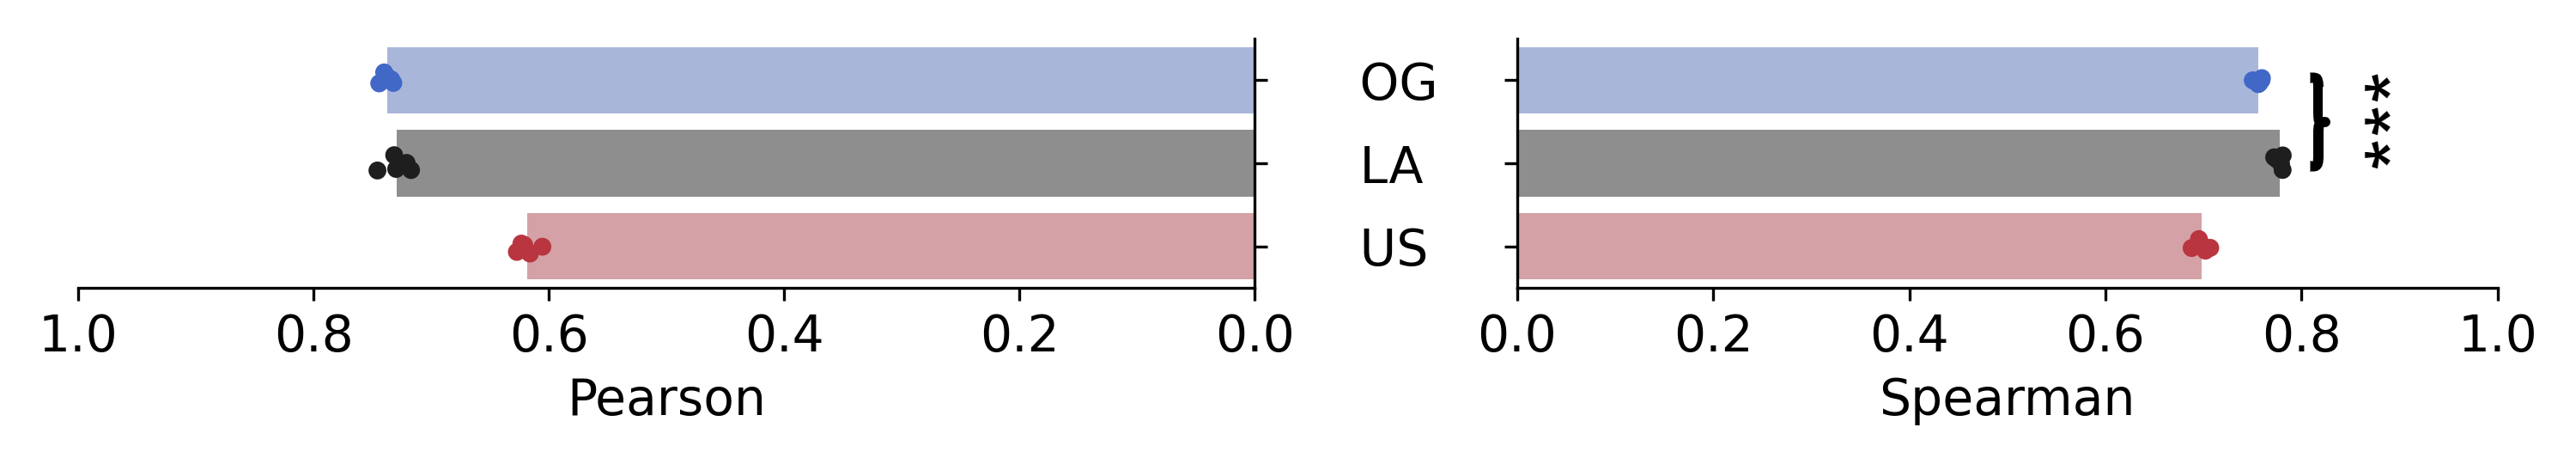
\includegraphics[width=0.8\textwidth]{adjustment-deepprime-dp-hek293t-performance.png}
        \label{fig:deepprime-dp-hek293t-adjustment-performance}
    }
    \vspace{-3mm} % Reduce vertical space between subfigures
    \subfigure[PD HEK293T]{
        \centering
        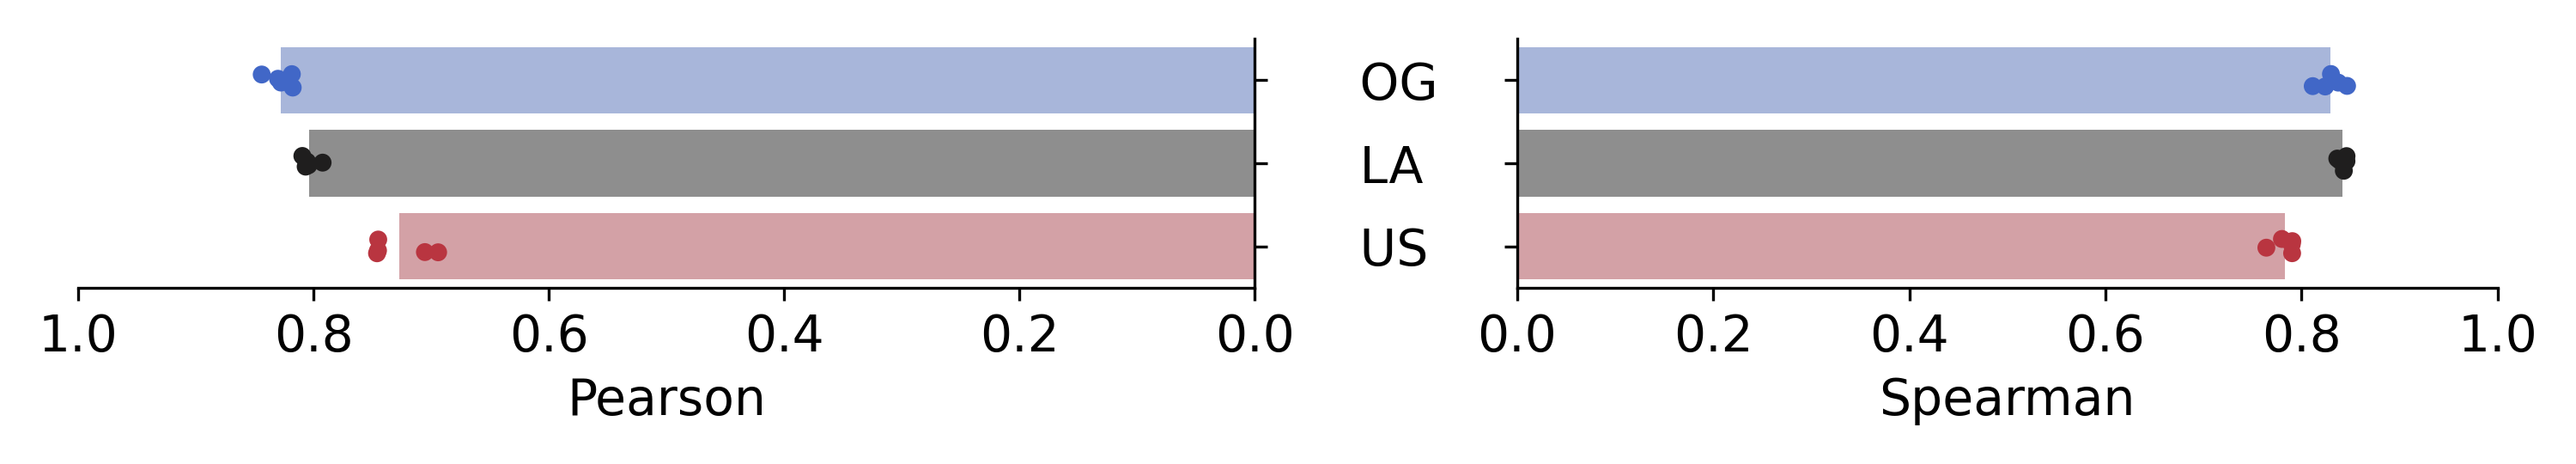
\includegraphics[width=0.8\textwidth]{adjustment-deepprime-pd-hek293t-performance.png}
        \label{fig:deepprime-pd-hek293t-adjustment-performance}
    }
    \vspace{-3mm} 
    \subfigure[PD K562]{
        \centering
        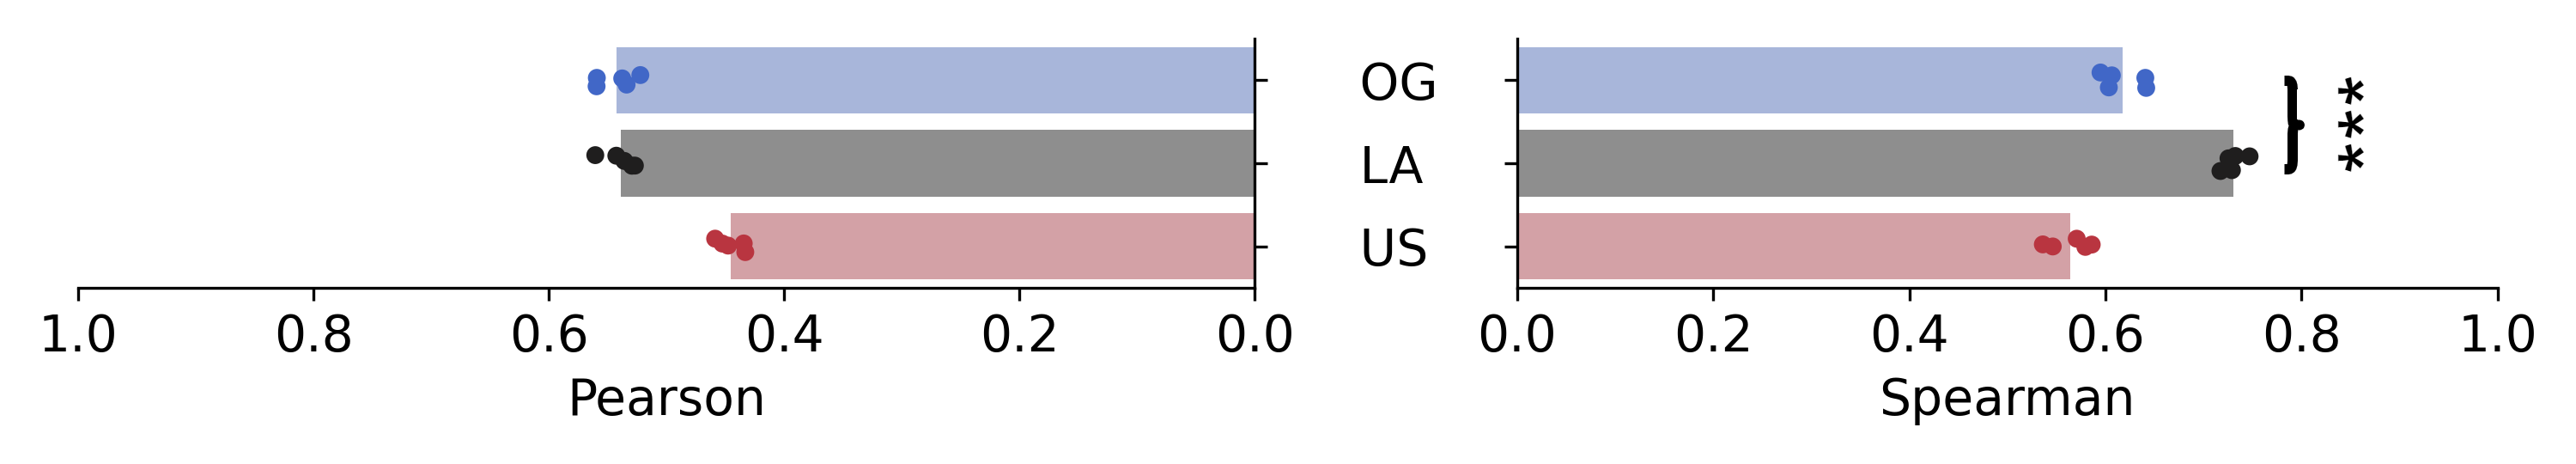
\includegraphics[width=0.8\textwidth]{adjustment-deepprime-pd-k562-performance.png}
        \label{fig:deepprime-pd-k562-adjustment-performance}
    }
    \vspace{-3mm} 
    \subfigure[PD K562MLH1dn]{
        \centering
        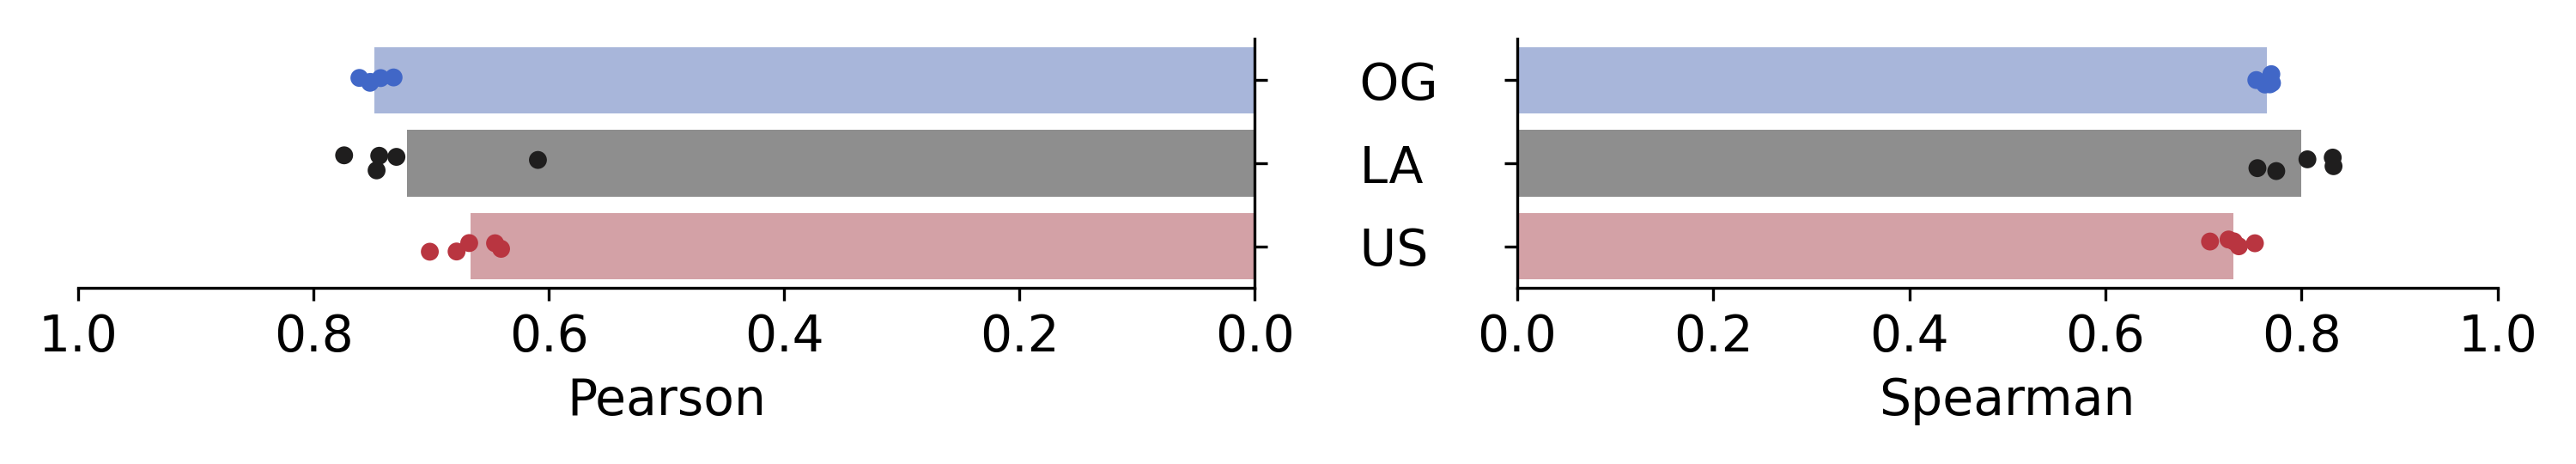
\includegraphics[width=0.8\textwidth]{adjustment-deepprime-pd-k562mlh1d-performance.png}
        \label{fig:deepprime-pd-k562mlh1d-adjustment-performance}
    }
    \vspace{-3mm} 
    \subfigure[PD Adv]{
        \centering
        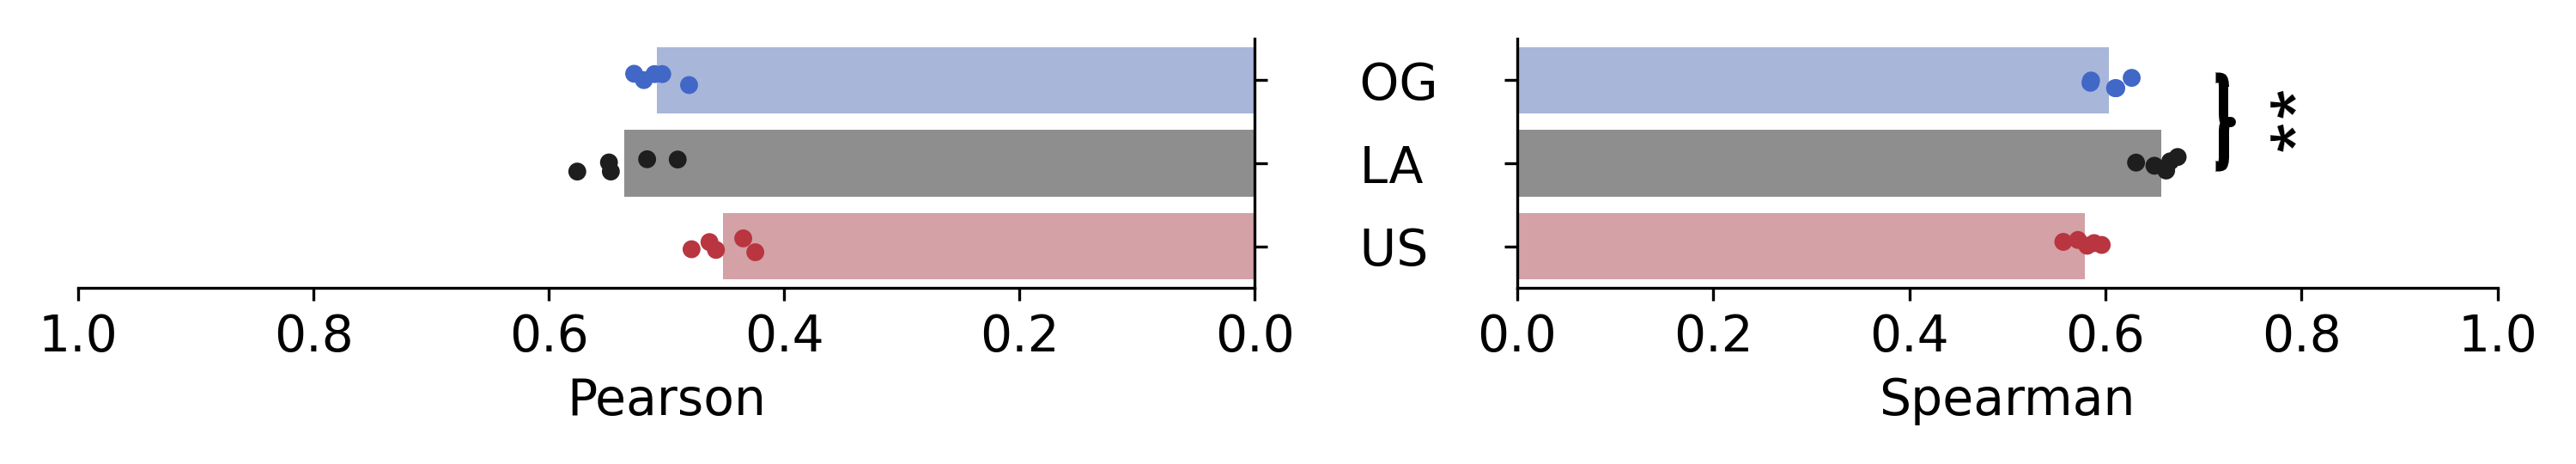
\includegraphics[width=0.8\textwidth]{adjustment-deepprime-pd-adv-performance.png}
        \label{fig:deepprime-pd-adv-adjustment-performance}
    }
    \caption[DeepPrime model performance comparison after adjustments]{
        Similar to \autoref{fig:adjustment-performance}, the performance comparison of the MLP model trained on the DeepPrime HEK293T PE2 dataset \textbf{(a)}, and the PRIDICT2.0 HEK293T dataset \textbf{(b)}, the PRIDICT2.0 K562 dataset \textbf{(c)}, the PRIDICT2.0 K562MLH1d dataset \textbf{(d)}, and the PRIDICT2.0 Adv dataset \textbf{(e)} using the log adjusted (LA), undersampled (US), and the original dataset (OG). 
    }
    \label{fig:deepprime-adjustment-performance}
\end{figure}

To further verify the necessity of the adjustments, the DeepPrime model with log adjusted and undersampled target were trained on the five datasets using the optimized hyperparameters reported by Yu et al in their study (detailed training process to be discussed in \autoref{sec:training-deepprime-pridict})\cite{yuPredictionEfficienciesDiverse2023}. The performance of the models were then evaluated using Pearson and Spearman correlation and compared to the result trained on the original model, shown in \autoref{fig:deepprime-adjustment-performance}.

As expected, the relative performance of the undersampling adjustment took a nosedive when training the DeepPrime model with far more parameters than the simple MLP model. Significantly lower performance was observed on all datasets ($p<0.01$) trained with undersampled training data. The log adjustment, on the other hand, showed a significant improvement in terms of Spearman's $\rho$ on the DeepPrime HEK293T dataset ($p<0.001$), the PRIDICT K562 dataset ($p<0.001$), and the PRIDICT Adv dataset ($p<0.01$). However, at the same time, significant decrease in performance was observed in terms of Pearson's R for the DeepPrime and PRIDICT HEK293T datasets ($p<0.05$). 

Taking into account the performance of the DeepPrime model, I decided to follow PRIDICT's protocol and not adjust the target values. 

Another problem with the dataset is the lack of variety in the PBS length and location in the PRIDICT dataset. For some reason, all PBS sequences start at 5bp downstream of the protospacer start location and have a length of 13bp, ending before the nick site at 3bp upstream of PAM. This can significantly impact the model's performance during inference on data with arbitrary PBS length and location, especially if PBS related features were directly used by the models. 

To help the models trained on PRIDICT datasets work on unseen data supplied by the users, the suggested PBS length is fixed at 13bp when inferencing using models trained on PRIDICT dataset, with PBS always starting at 5bp downstream of the protospacer start location.



\section{Determinants of Prime Editing Outcome}
\label{sec:determinants}

\begin{figure}
    \centering
    \subfigure[DeepPrime]{
        \label{fig:shap-dp-pe2-hek}
        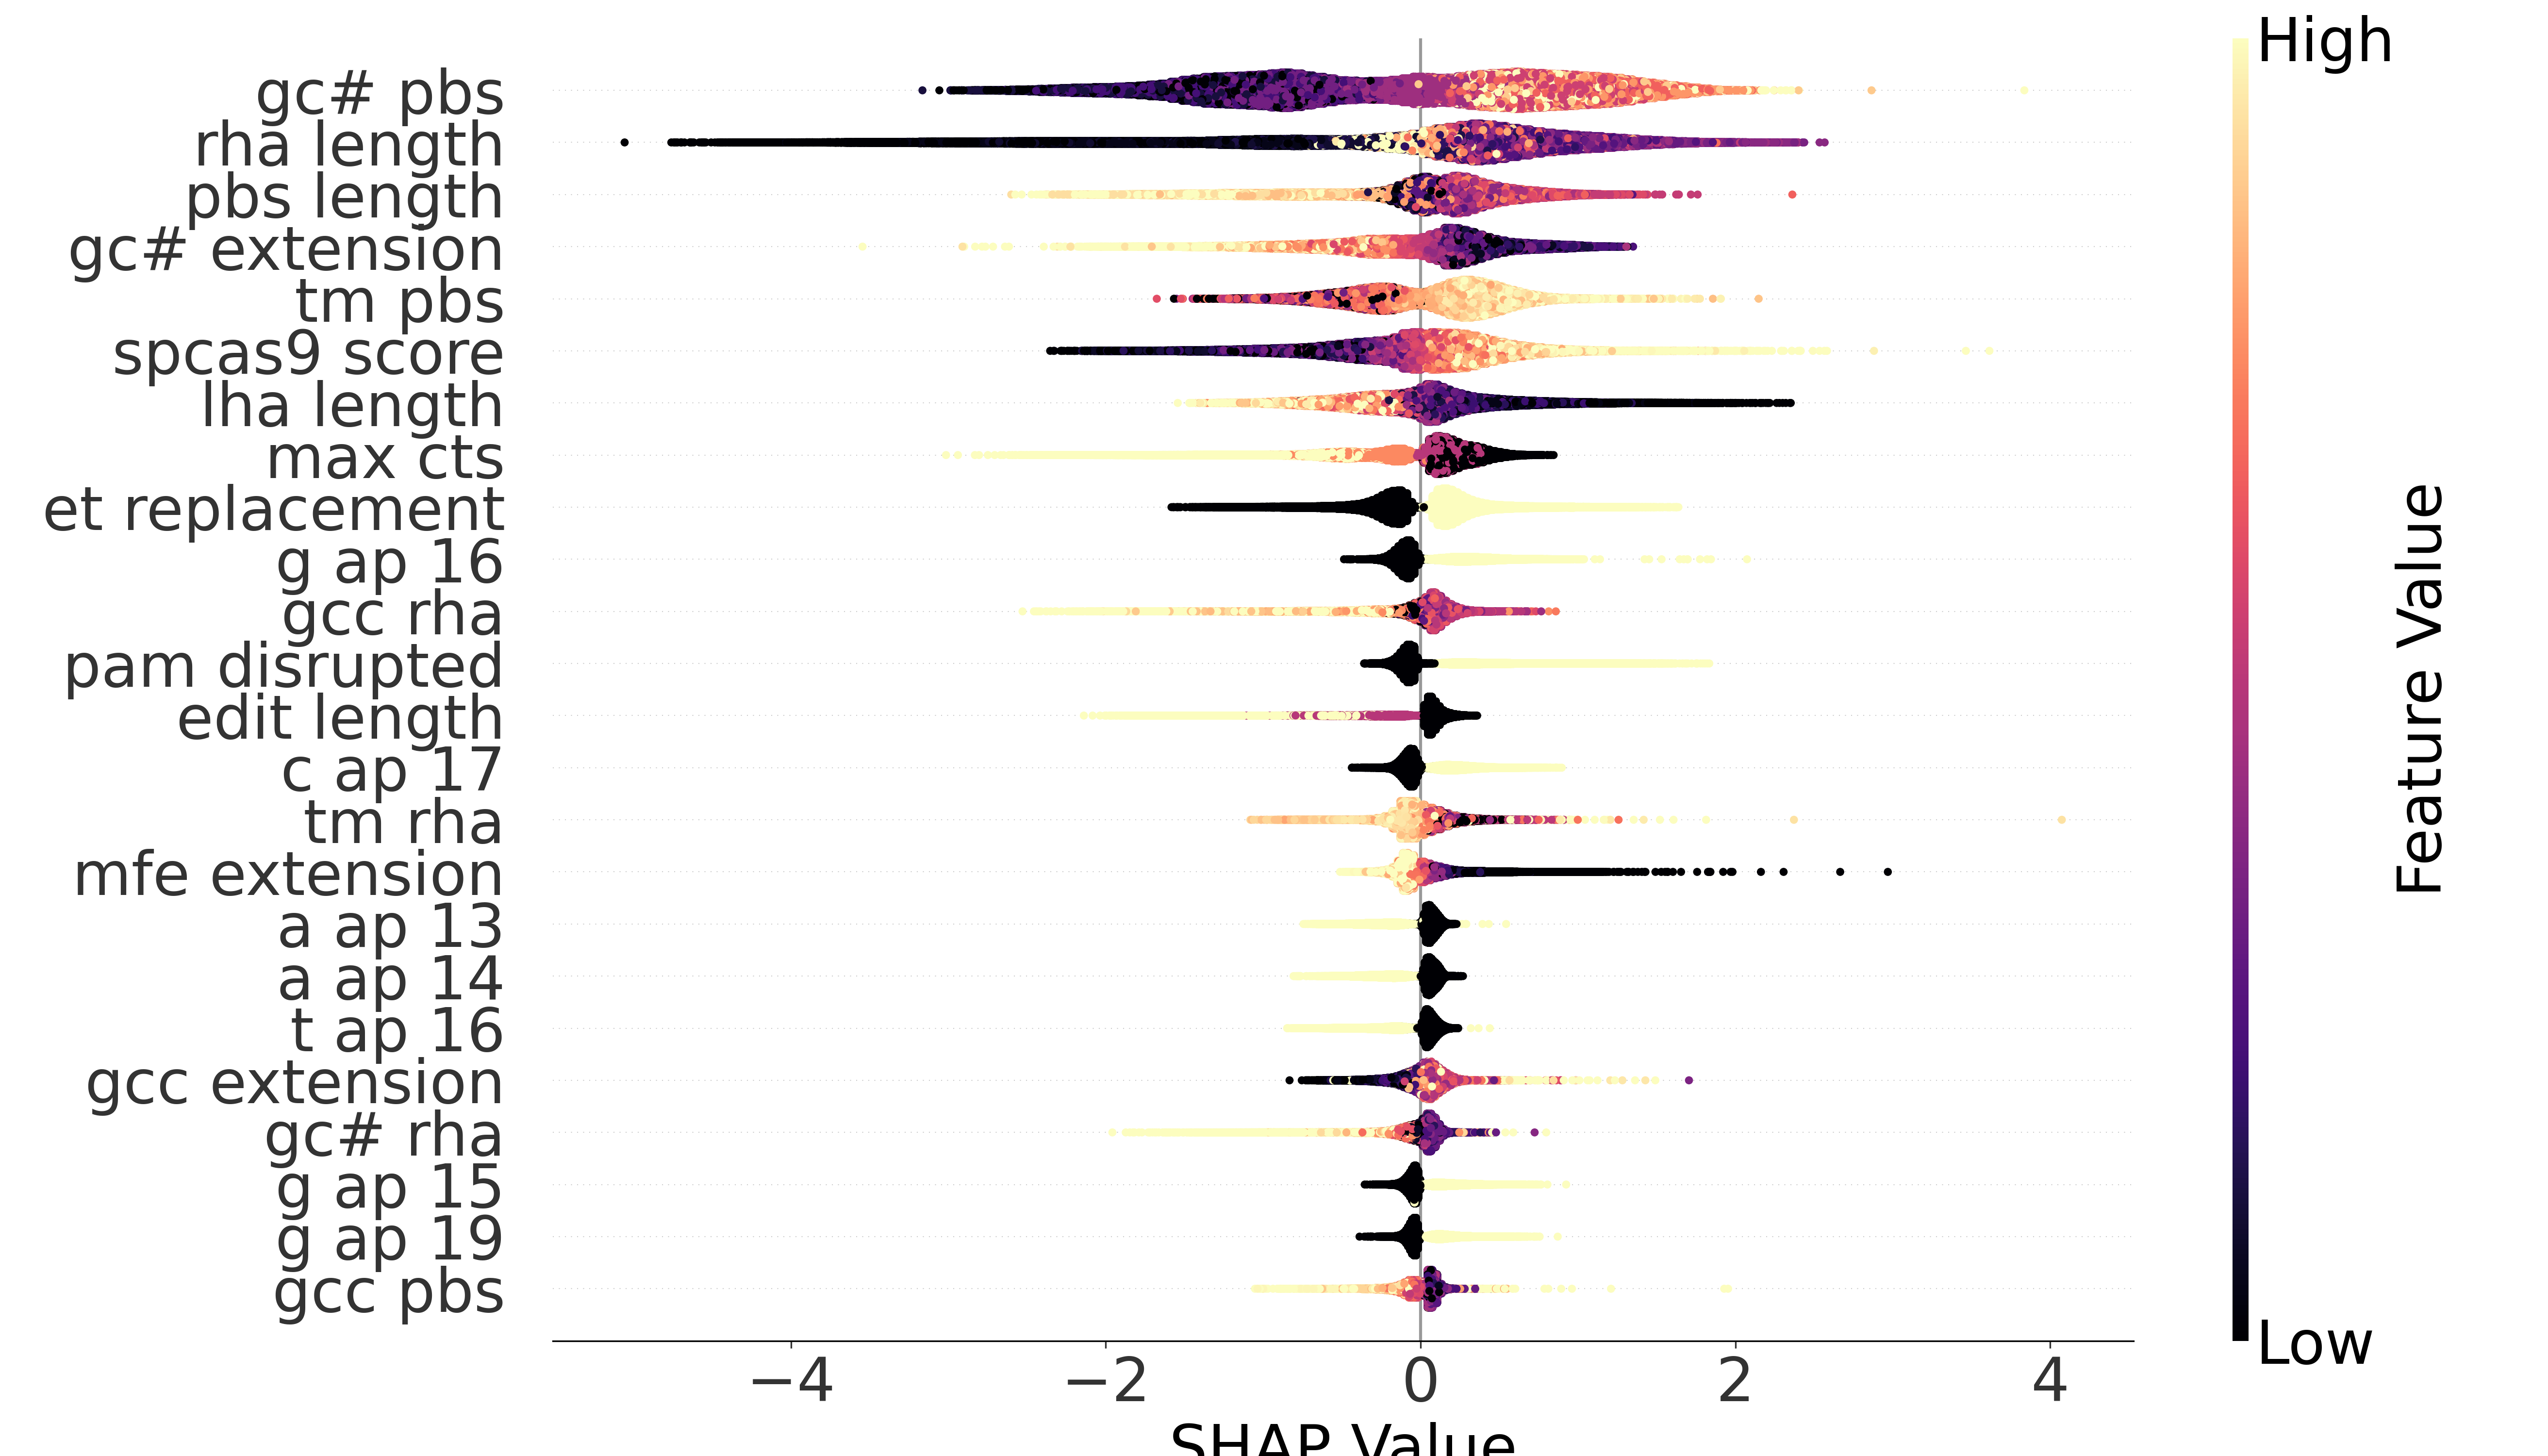
\includegraphics[width=0.99\textwidth]{shap-dp-hek293t-pe2.png}}
    \subfigure[Deletion]{
        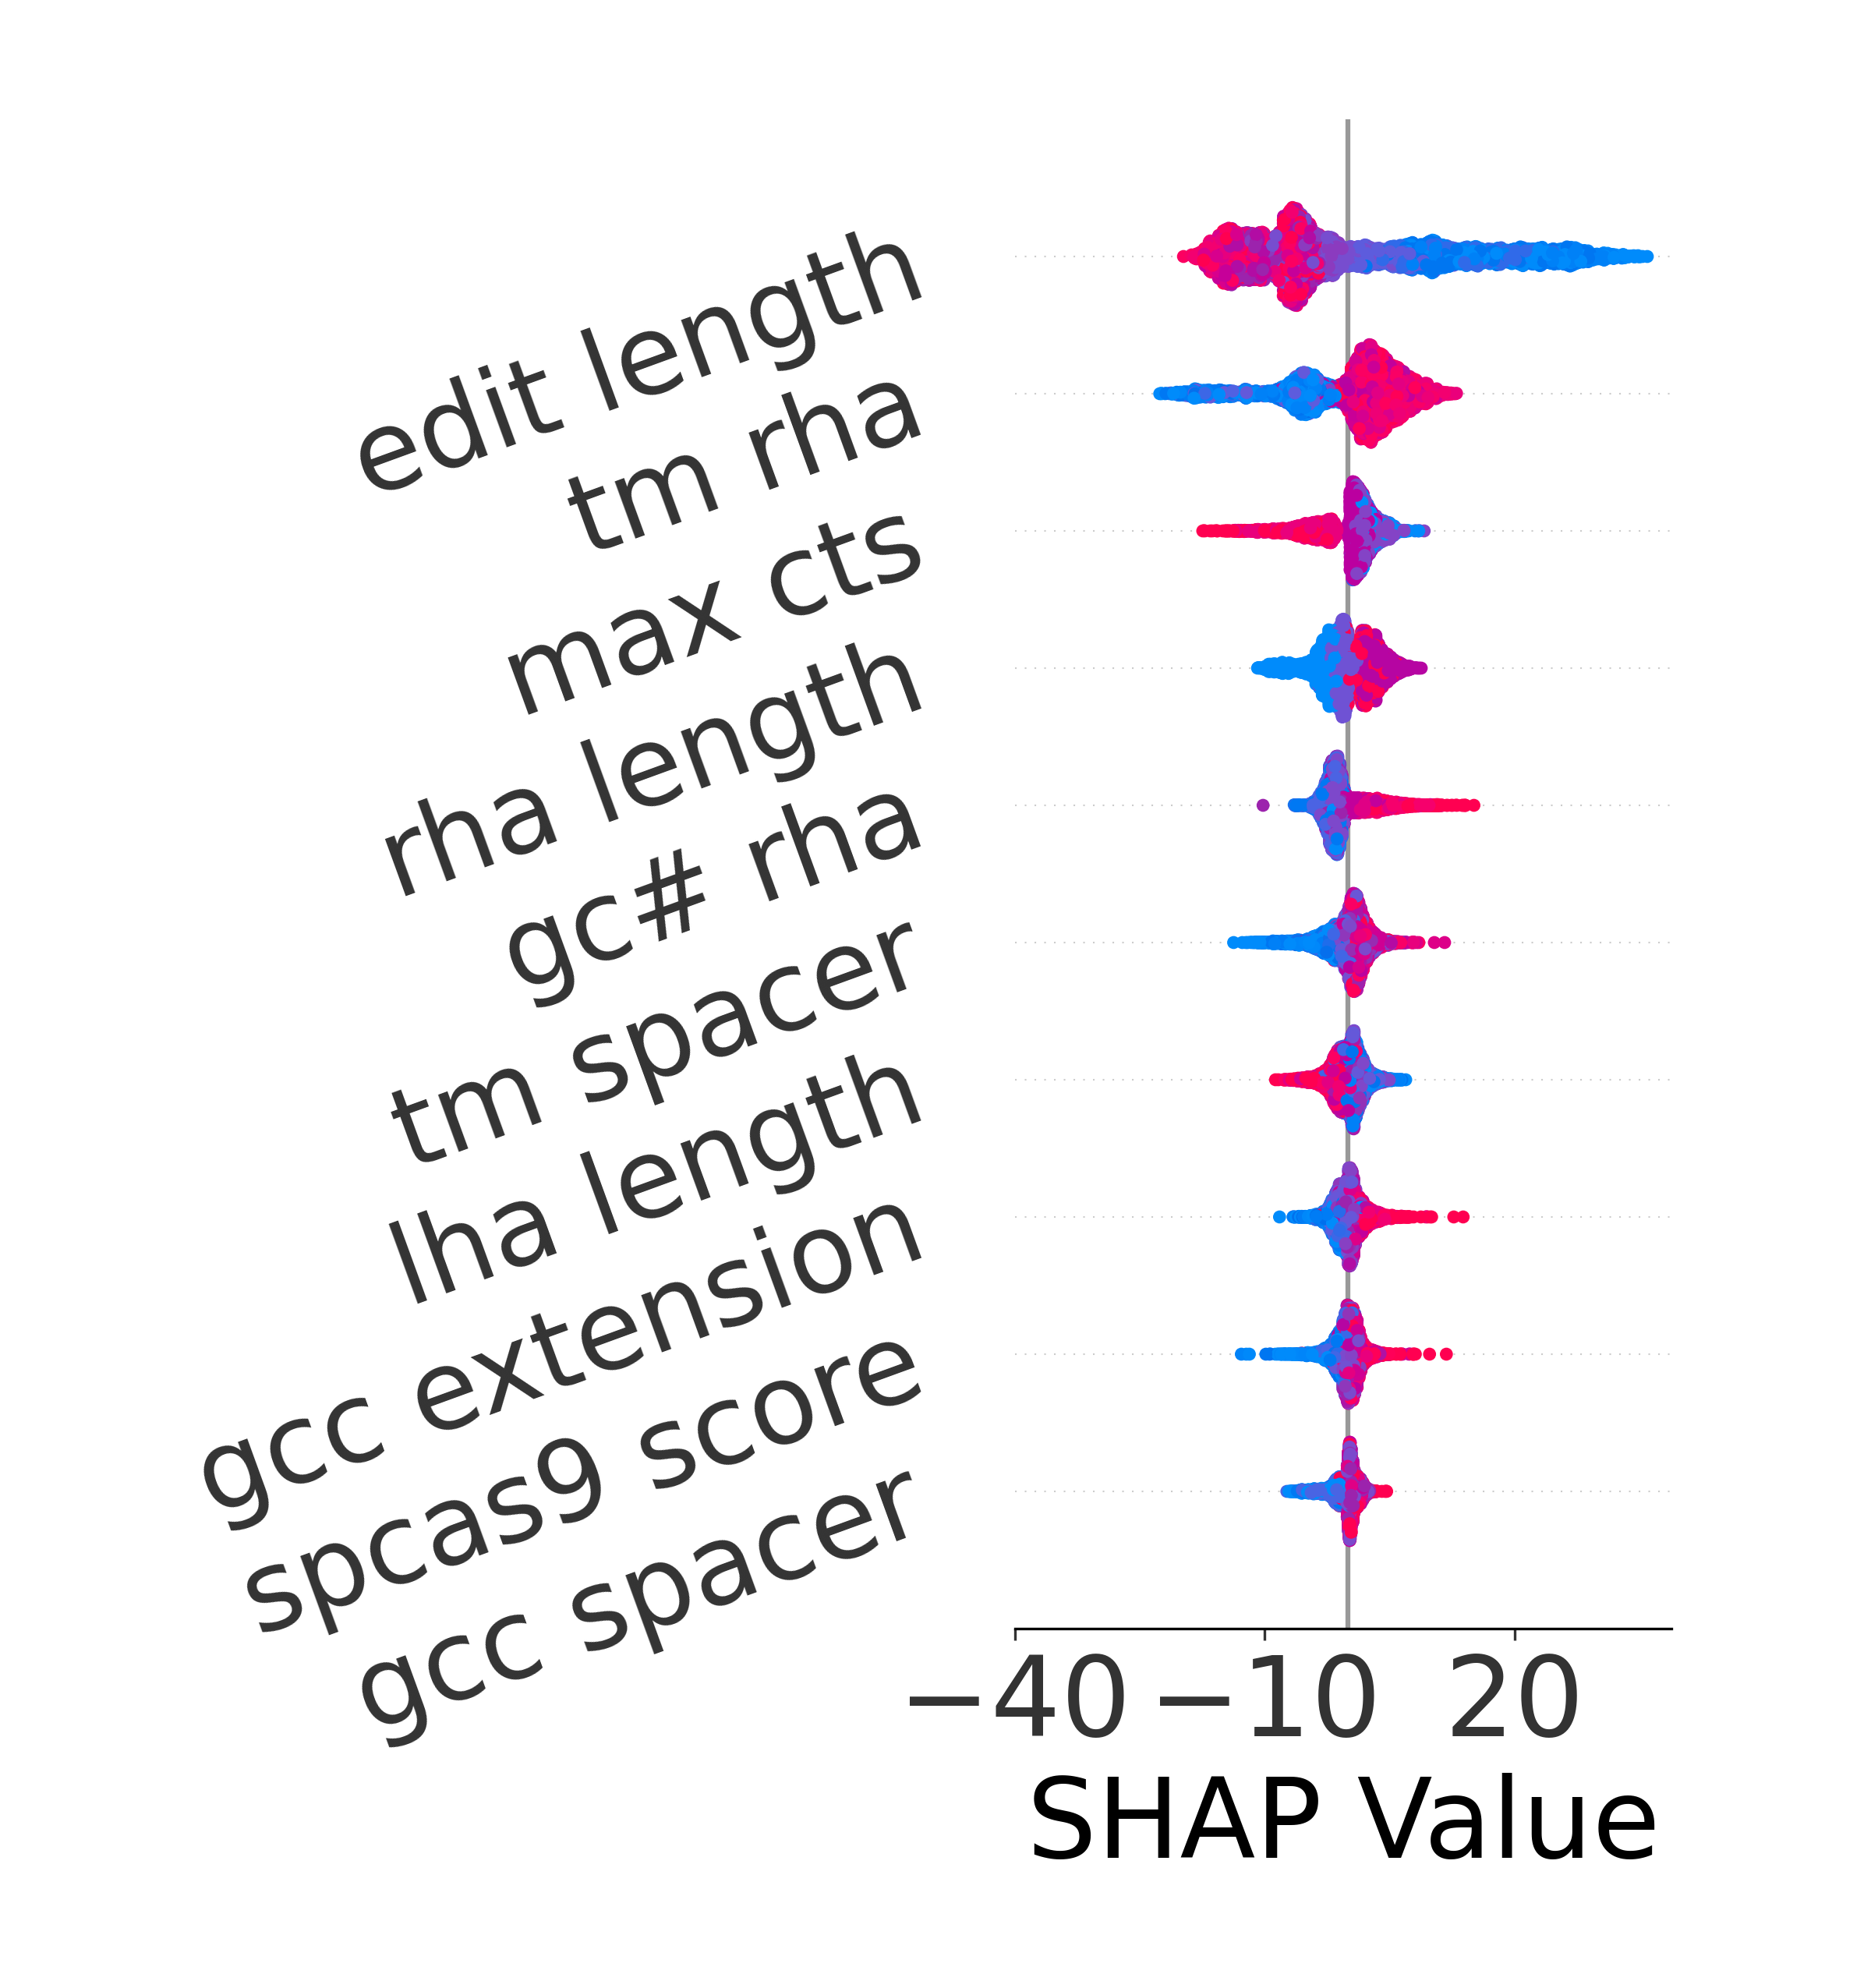
\includegraphics[width=0.3\textwidth]{shap-pd-hek293t-pe2-delete.png}
    }
    \subfigure[Insertion]{
        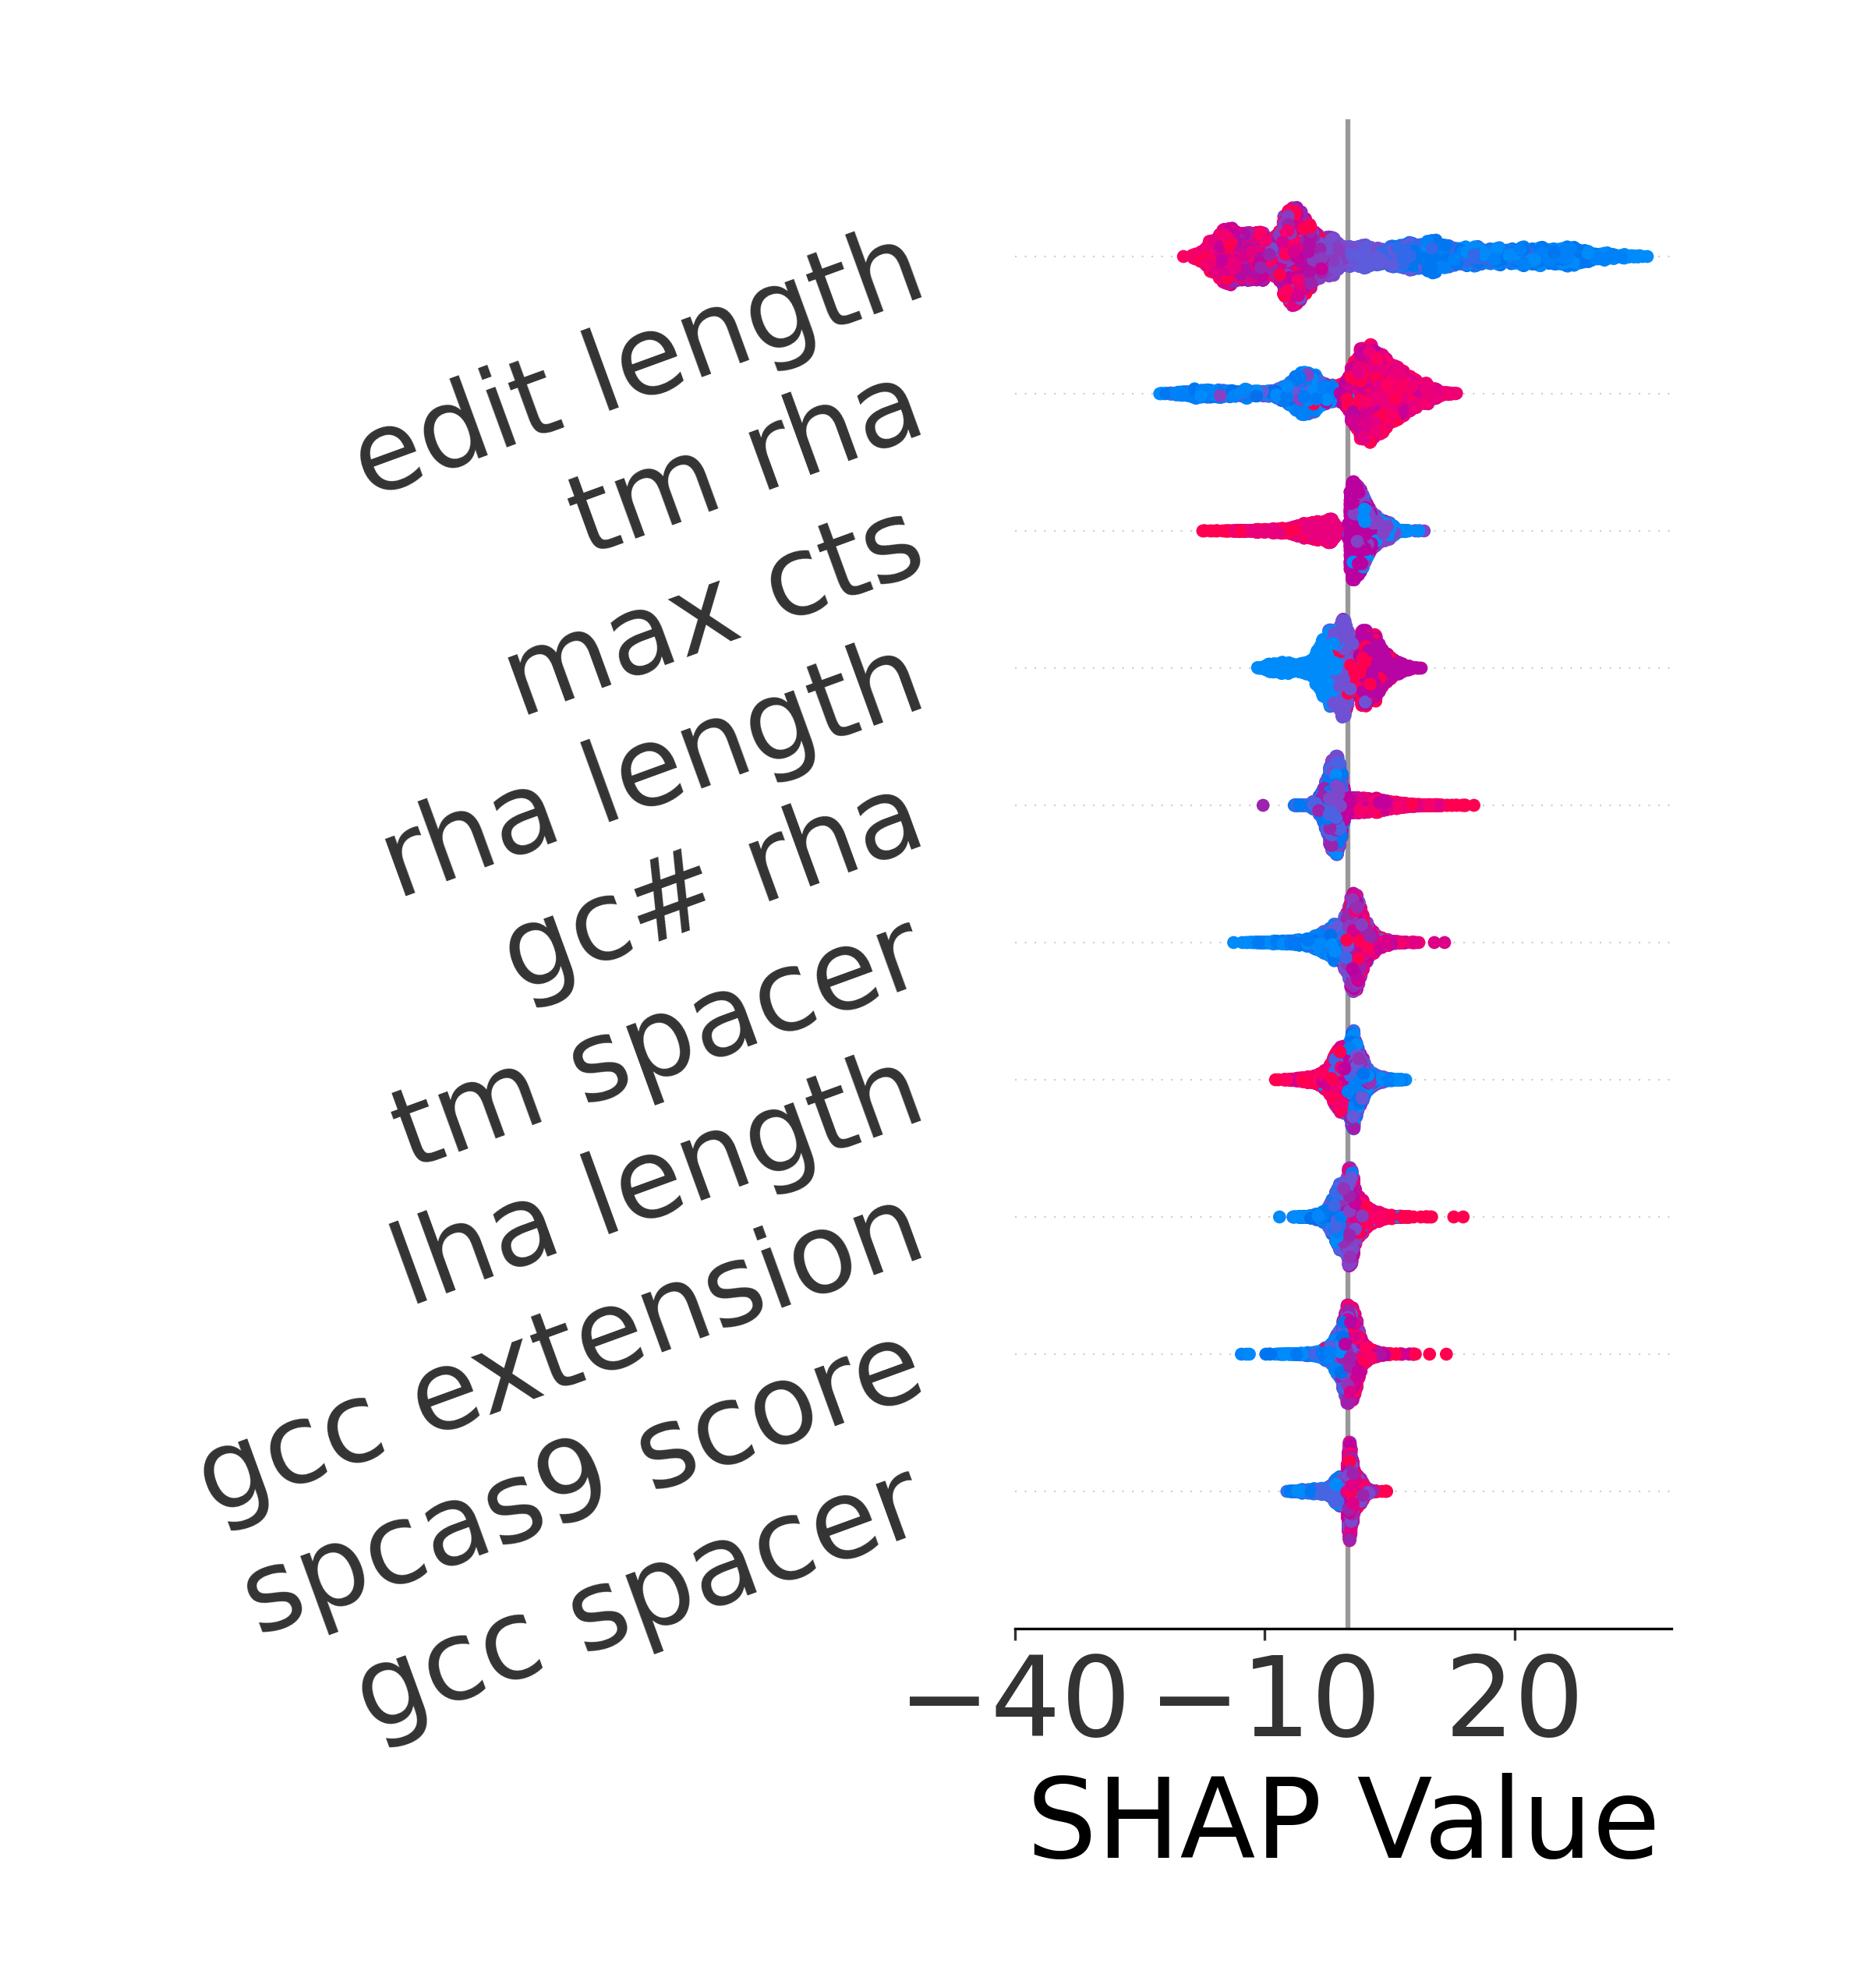
\includegraphics[width=0.3\textwidth]{shap-pd-hek293t-pe2-insert.png}
    }
    \subfigure[Replacement]{
        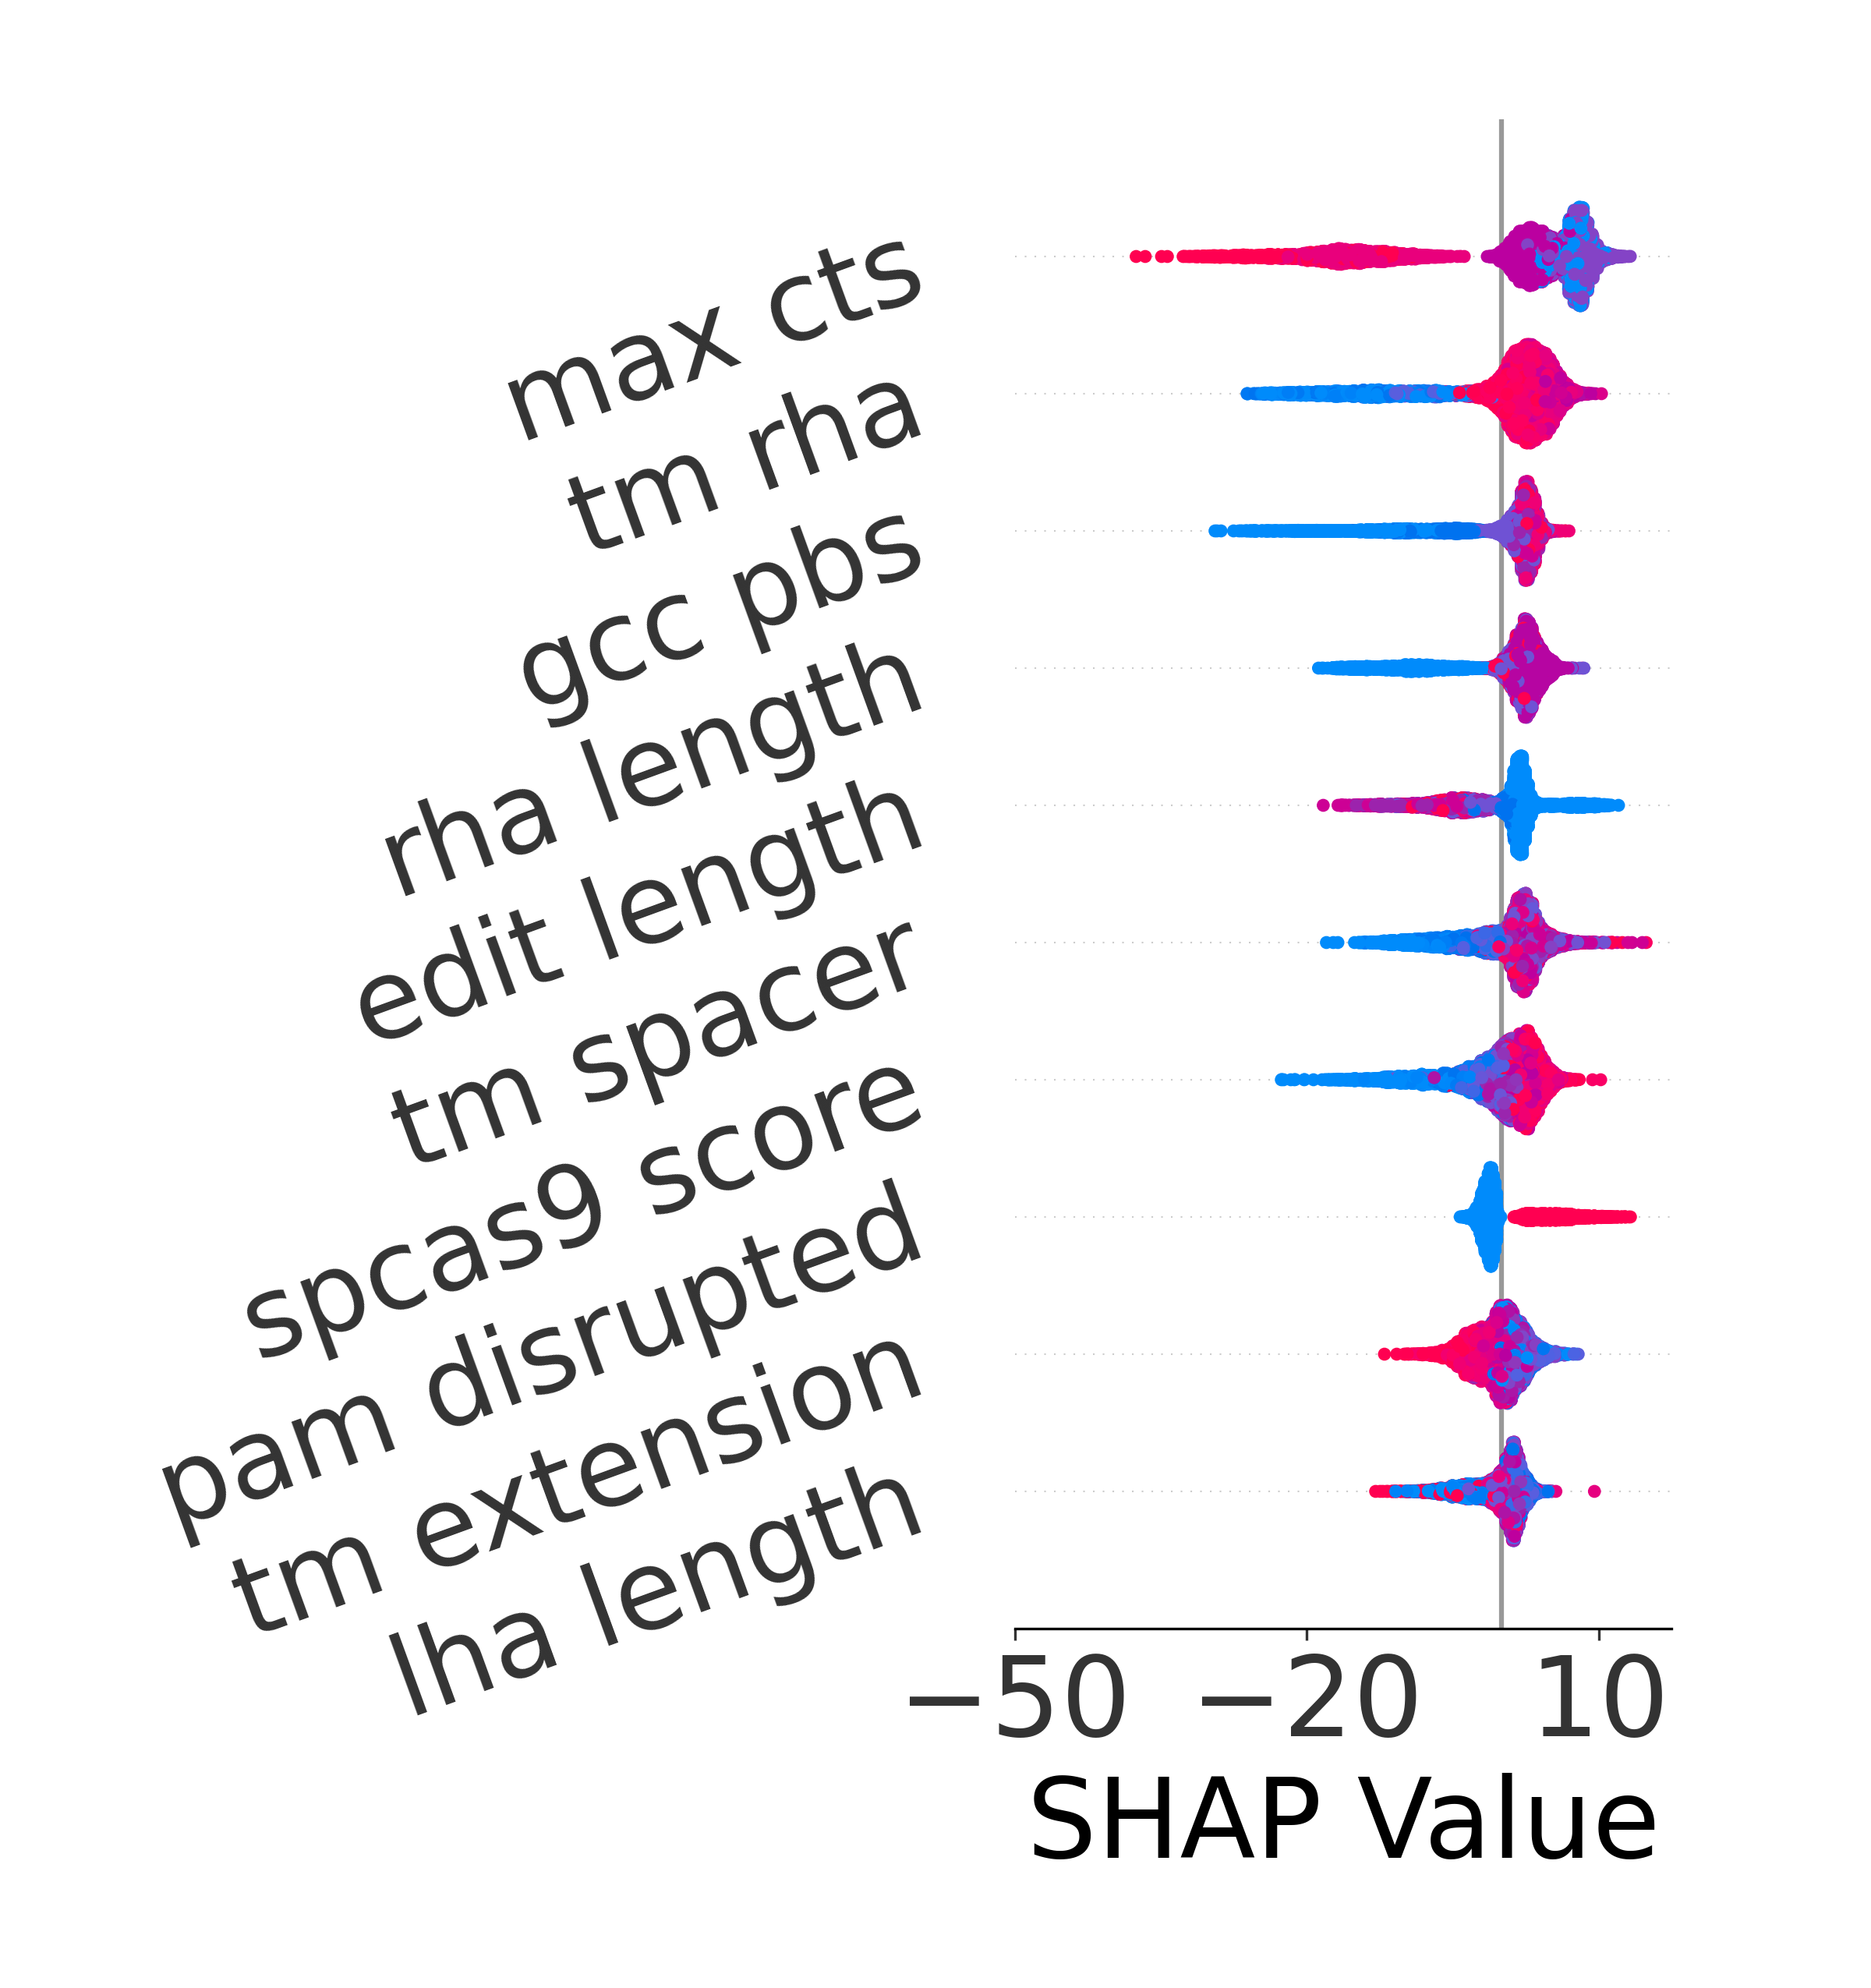
\includegraphics[width=0.3\textwidth]{shap-pd-hek293t-pe2-replace.png}
    }
    \caption[SHAP analysis for DeepPrime and PRIDICT2.0 datasets on HEK293T cell line.]{SHAP analysis for DeepPrime and PRIDICT2.0 datasets on HEK293T cell line: \textbf{(a)} Top 15 determinants from SHAP analysis using all of DeepPrime HEK293T Datasets. \textbf{(b-d)} Top 10 determinants from SHAP analysis using PRIDICT2.0 HEK293T data for each individual editing types. The colour of the individual data point shows their normalized values from high (red) to low (blue). The binary values have 1 (True) for high and 0 (False) for low. A number of shorthands have been used to improve the clarity of the illustrations. gcc for GC Content (different from GC count); et for editing type; tm for melting temperature; mfe for minimum free energy; n ap \# for base n at protospacer position \#; max cns for the length of maximum consecutive sequence of base n.} 
    \label{fig:shap}
\end{figure}

As discussed in \autoref{sec:motivation}, most of the recent deep learning models surveyed in the literature (DeepPrime\cite{yuPredictionEfficienciesDiverse2023} and PRIDICT\cite{mathisPredictingPrimeEditing2023,mathisMachineLearningPrediction2024}) followed a similar two model structure. The first model is a deep neural network taking in raw sequence data, and the second model is a smaller MLP/regression model that takes as input the features extracted from the PBS, RTT and ngRNA. For single model architecture (DeepPE\cite{kimPredictingEfficiencyPrime2021}), the features are concatenated to the sequence data and fed into the model.

As a result, it is important to find the most prominent determinants of prime editing outcomes and to extract the most informative features for describing the pegRNA. A large number of features were selected from various sources as the studies focus on different aspects of pegRNA. Shapley Additive Explanations (SHAP) with XGBoost regressor to rank the features based on their importance. The full list of features investigated can be found in \autoref{appendix:features}. 

A number of Python libraries were utilized when extracting the features into the `shap' format. The melting temperature of the sequences were calculated using the 'biopython' library\cite{cockBiopythonFreelyAvailable2009}, the minimum free energy was calculated with the ViennaRNA package and adjusted using sequence length to ensure it's mostly influenced by sequence's nucleotide order and composition\cite{lorenzViennaRNAPackage2011,trottaNormalizationMinimumFree2014}, and the SpCas9 scores were provided by the 'DeepSpCas9' model\cite{kimSpCas9ActivityPrediction2019}. Other features such as GC content were extracted using simple Python string processing functions.

SHAP analysis was first conducted on the largest DeepPrime PE2 HEK293T dataset to provide the most robust identification of the most informative features (Figure \ref{fig:shap-dp-pe2-hek}). The features were then sorted based on their importance, and the top 24 features were used for the model, matching the design optimized by DeepPrime\cite{yuPredictionEfficienciesDiverse2023}. To identify the influence of the features on different editing types, SHAP analysis was also conducted on the PRIDICT2.0 HEK293T dataset for each individual editing type (\autoref{fig:shap}(b-d)), due to its higher variety of editing length. 

The major determinants are as follows:
\begin{itemize}[itemsep=-0mm]
    \item \textcolor{red}{Editing type and length}: editing type has a significant impact on the editing efficiency, with the replacement type having higher efficiency than the insertion and deletion, as shown by the `et replacement' feature in Figure \ref{fig:shap-dp-pe2-hek}. The length of the edit also has great influence on editing result, and its important is more pronounced for deletions and insertions than replacements. As expected, longer edits have lower efficiency due to the increased difficulty in the annealing and repair process.
    \item \textcolor{red}{Melting temperature}: melting temperature (Tm) refers to the temperature at which half of the RNA strand become unfolded or denatured. It is strongly correlated with the editing efficiency, possibly due to its influence on RNA structural stability. Its actual effect, however, is highly mixed. A low Tm in extension seems to positively affect the editing result, while the opposite is true for pbs. At the same time, high Tm in RHA has a mixed impact in the DeepPrime dataset (`tm rha' in Figure \ref{fig:shap-dp-pe2-hek}), while in the PRIDICT2\.0 dataset, high Tm in the PBS is clearly beneficial for the editing process of all types (`tm rha' in \autoref{fig:shap}(b-d)).
    \item \textcolor{red}{Minimum free energy}: minimum free energy (MFE) describes the lowest possible energy required for a RNA sequence to stay in a particular form\cite{lorenzViennaRNAPackage2011}. It appears to have similar effect to Tm, with low MFE in the extension being beneficial for the editing efficiency.
    % TODO: Check MFE 
    \item \textcolor{red}{GC content/count}: GC count in the PBS sequence was shown to be the most important feature for the DeepPrime dataset (Figure \ref{fig:shap-dp-pe2-hek}), consistent with the observation made by Liu et al in their 2019 study introducing prime editors\cite{liudavidr.SearchandreplaceGenomeEditing2019}. They expected lower editing efficiency with low GC count in the PBS, due to the energetic requirements of hybridization of the nicked DNA strand to the PBS. GC content also correlates to the minimum free energy and melting temperature, as GC base pairs have stronger hydrogen bond than AU base pairs.
    \item \textcolor{red}{Poly-T sequences}: Shown as `max cts' in \autoref{fig:shap}, the length of the longest consecutive T (poly-T) sequences in the cDNA of the 3'extension and spacer RNA sequences has a clear negative impact on the editing efficiency. The poly-T termination signal, while not causing termination in itself, causes catalytic inactivation and backtracking of Pol III\cite{nielsenMechanismEukaryoticRNA2013}
    \item \textcolor{red}{SpCas9 score}: DeepSpCas9 is a deep learning model that estimates the activity of the SpCas9 protein on a target loci, and has been shown to be a good indicator of prime editing efficiency\cite{kimPredictingEfficiencyPrime2021}. This is likely due the SpCas9's role in the prime editing process, as it is responsible for the initial binding of the pegRNA to the target loci. 
    \item \textcolor{red}{PAM disruption}: it was shown that prime editors can sometimes rebind to the edited sequences and induce unintended edits, lowering the editing efficiency\cite{liudavidr.SearchandreplaceGenomeEditing2019}. Thus, the disruption of the PAM sequence is beneficial for the editing efficiency as it prevents the reannealing of the pegRNA to the edited sequence.
    \item \textcolor{red}{LHA/RHA/PBS length}: the length of rha (right homology arm, RTT overhang) is a significant determinant for all editing types, with a short rha length leading to deceased prime editing efficiency, while the positive effect of a long rha is not as pronounced. This suggests the existence of a minimum threshold for rha length below which the edited strand cannot efficiently anneal to the unedited strand, consistent with the findings of Yu et al, 2023, recommending a rha length of at least 7nt\cite{yuPredictionEfficienciesDiverse2023}. Reported as edit position in some literatures, lha length corresponding to the distance between the PAM sequence and the edit location is also a significant feature for all editing types, especially insertion and deletion. A longer lha length adversely affects the editing efficiency, suggesting that although prime editors have less stringent requirements for PAM locations, editing should still be done close to the protospacer whenever possible. As for PBS length, both a very short and a very long PBS have a negative impact on the editing efficiency, suggesting an optimal range.
    \item \textcolor{red}{Protospacer nucleotide composition}: in Figure \ref{fig:shap-dp-pe2-hek}, a guanine nucleotide (G) at protospacer location 16 was shown to have a positive impact on the editing efficiency. On top of that, among the top 24 features, the nucleotide compositions from protospacer location 13 to 17 were all shown to have a significant impact. 
    
    This is consistent with Mathis et al's finding that the nucleotide composition from protospacer position 10 to 20 shows high integrated gradient scores, suggesting that the nucleotide composition in this region is highly influential in determining the editing efficiency\cite{mathisPredictingPrimeEditing2023}.
    % TODO explain why
\end{itemize}

On top of the quantitatively invested sequence based features, higher level features have also been shown to impact prime editing efficiency:
\begin{itemize}[itemsep=-0mm]
    \item \textcolor{red}{pegRNA secondary structure}: the secondary structure of the pegRNA can impact the efficiency by inducing degradation of the 3' extension. The defunct pegRNA can still combine with target loci using its functioning 5' ngRNA, thus lowering the editing efficiency\cite{nelsonEngineeredPegRNAsImprove2022}.
    \item \textcolor{red}{MMR Behaviour}: as briefly mentioned at the beginning of \autoref{sec:prime-editing-process}, the mismatch repair(MMR) system adversely affects the editing efficiency during step (e) of the prime editing process. The MMR system may reject the annealing of the editing strand to the target loci, or it may excise the edited sequence, preferring the original sequence\cite{chenEnhancedPrimeEditing2021}. 
\end{itemize}

These features are encapsulated in the editing cell type and PE version and are thus not explicitly included in the feature list. For example, epegRNAs(engineered pegRNA) are improved version of pegRNA that are designed for protection against 3' erosion with a more robust secondary structure than the original versions\cite{nelsonEngineeredPegRNAsImprove2022}. At the same time, PE4 and PE5 are newer versions of prime editors with MLH1dn proteins that can suppress the MMR system\cite{chenEnhancedPrimeEditing2021}, and the HEK293T cell line has weaker MMR activity than other cell lines such
as HAP1(derived from a chronic myelogenous leukemia patient)\cite{mathisPredictingPrimeEditing2023}. 


\section{Conventional Machine Learning Models}
\label{sec:conventional-ml}

Using the top 24 computed features, a number of conventional machine learning models were trained to serve as a baseline for the deep learning models. The models include Lasso and Ridge regression, Random Forest Regressor, Gradient Boosted Trees from the XGBoost library, and a Multi-Layer Perceptron.

Their hyperparameter were optimized on one fold of the DeepPrime HEK293T using sklearn's GridSearchCV function, following the protocol used by PRIDICT. The performance of the optimized models were then evaluated using Pearson and Spearman correlation on the DeepPrime and PRIDICT dataset for three different cell types on all 5 folds to provide a more accurate estimation of the models' performance. The MLP model involved the additional Skorch library to allow for the use of scikit-learn's GridSearchCV for hyperparameter optimization on the Pytorch model. The optimized parameters for the models are as follows:

\begin{itemize}[itemsep=-0mm]
    \item \textcolor{blue}{Lasso}: \verb|alpha=0.006158482110660266| (coefficient for penalty term for L1 regularization)
    \item \textcolor{blue}{Ridge}: \verb|alpha=494.17133613238286| (coefficient for penalty term for L2 regularization)
    \item \textcolor{blue}{Random Forest}: \verb|n_estimators=200| (number of trees to build), \verb|max_depth=10| (maximum depth of the trees)
    \item \textcolor{blue}{XGBoost}: \verb|n_estimators=200| (number of boosting rounds, similar to number of trees), \verb|max_depth=5| 
    \item \textcolor{blue}{MLP}: \verb|hidden_layer_sizes=(64, 64)| (two hidden layer with 64 units each), \verb|activation='relu'| (rectified linear unit activation), \verb|solver='adam'| (adaptive moment estimation solver), \verb|lr=0.005| (learning rate)
\end{itemize}

When training the models, the MLP makes a futher validation set in the training data to prevent overfitting and improve the model's generalization. However, since sklearn does not offer a monitor for validation loss, the other models were fitted using the entire training data and trained until convergence.

The models' performance were evaluated using Pearson and Spearman correlation between predicted and measured efficiency, and the result of the conventional models on the four datasets were shown in \autoref{fig:conventional_ml_models_performance}. 

Although similar in accuracy, XGBoost's gradient boosted trees have far superiour efficiency compared to the Random Forest model thanks to its GPU support and optimized implementation ($\sim$300 times faster).

\begin{figure}
    \centering
    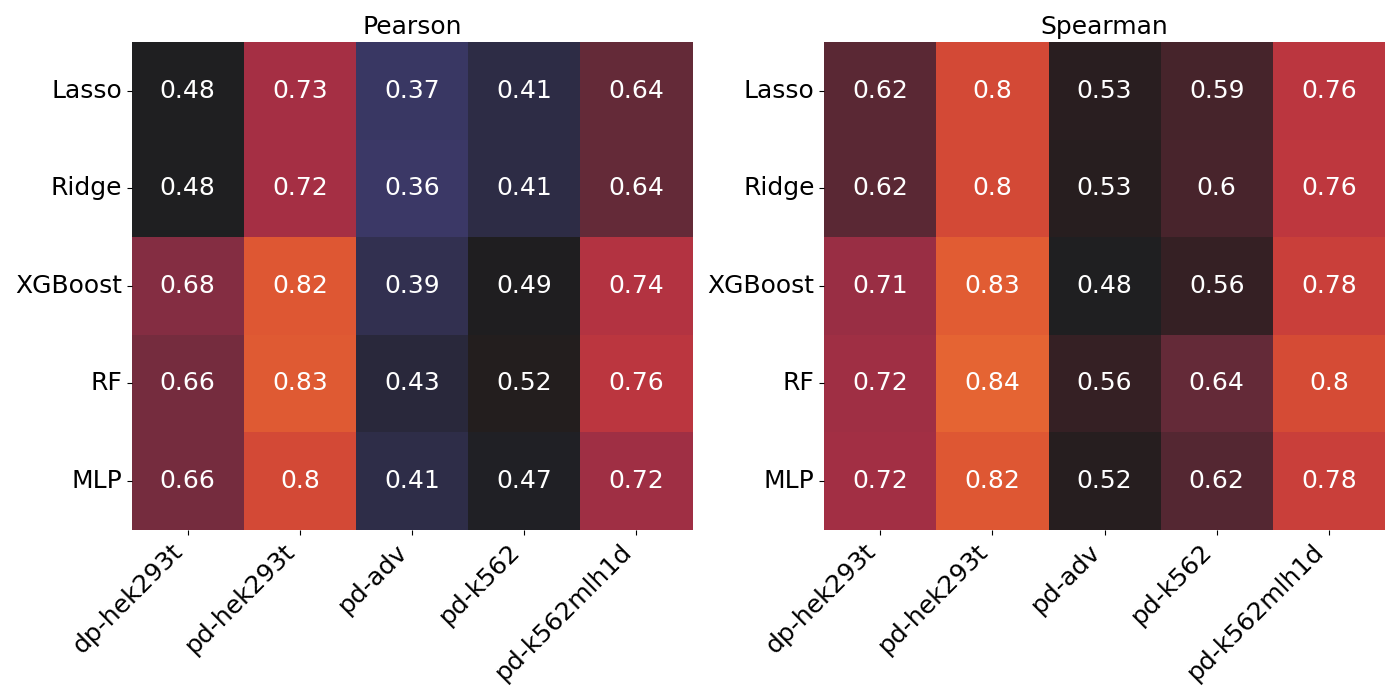
\includegraphics[width=0.8\textwidth]{conventional_ml_models_performance.png}
    \caption[Conventional ML model performance comparison]{Performance compaison in terms of Pearson's r (\textbf{left}) and Spearman's R (\textbf{right}) for a number of conventional machine learning models on the DeepPrime HEK293T PE2 dataset and the PRIDICT2.0 datasets for three different cell lines. The models are Multi-Layer Perceptron(MLP), Random Forest Regressor(RF), Lasso, Ridge, and XGBoost. The performance of the models were evaluated using mean of 5-fold cross validation. The heatmap were mapped to the same scale of [0, 1] for easier comparison.}
    \label{fig:conventional_ml_models_performance}
\end{figure}


\section{Improving Performance with Ensemble Learning}

The performance of the deep learning models can be further improved by using ensemble learning. The idea behind ensemble learning is to combine multiple models to produce a more accurate prediction than any individual model. 

Ensemble learning is a common practice in machine learning, and is frequently seen in the top performing models in competitions hosted by Kaggle.
Most of the models tested in this study so far are already using ensembling learning. Random forrest trains multiple decision trees using a subset of features and samples to alleviates the problem of overfitting. The XGBoost model is anpther ensemble of multiple decision trees using gradient boosting, while DeepPrime, PRIDICT and the Transformer model are effectively an ensemble of a deep learning model and a MLP, using another MLP as a meta learning to combine the representation produced by the two base models.

In this study, a number of common supervised ensemble learning methods were evaluated, including weighted averaging, bagging, and adaptive boosting (AdaBoost). Due to the large number of models used in the ensemble, the initial training and testing were conducted on the same subset of the PRIDICT2.0 HEK293T dataset used for the hyperparameter tuning of the LLM model.

Bagging and  AdaBoost are normally used with estimators of the same type, but in this study, I wanted to utilize the strengths of different models to produce a possibly more accurate prediction. Thus, an additional meta learner similar to the ones used in the deep learning models was added to the ensemble models. The meta learner takes the prediction of the individual models as well as the 24 extracted features as input and produces the final prediction.

To first test their validity in this task before moving on to more sophisticated models, the models making up the ensemble are the conventional ML methods evaluated in \autoref{sec:conventional-ml}. Methods that achieved significantly higher performance than the individual models were then tested on the deep learning models.

% TODO: error distribution of the models

\subsection{Training DeepPrime and PRIDICT}
\label{sec:training-deepprime-pridict}

To begin with, for using the DeepPrime and PRIDICT models in the ensemble, the models need to be retrained on all datasets used in this study. A training script was written for each model with the help of Skorch wrapper, similar to the one used by the MLP model. The scripts loads the dataset, perform data conversions, and train the model using the hyperparameters optimized by the original authors. The hyperparameters selected by DeepPrime were listed in their study, while the parameters for PRIDICT were acquired by loading the pickled trained model's configuration. 

To verify the correctness of my implementation, I trained the models on their respective datasets and evaluated the performance. The features calculated for their models are listed in (Add appendix reference). The DeepPrime model achieved slightly lower performance than the one reported by Yu et al, with a mean pearson's correlation of 0.75 on the DeepPrime HEK293T PE2 dataset, compared to the 0.77 reported in their study. PRIDICT also achieved slightly lower Spearman's correlation on the PRIDICT HEK293T dataset, with a mean of 0.81 compared to the 0.82 reported by Mathis et al. These differences could be a result of different seed used for train val split used during training on each fold, or specific details of the training process, for example the parameters used by learning rate scheduler or the optimizer. 

After verifying the correctness of the model implementation, to remove the added variance of feature selection, all models were reconfigured to use the top 24 features extracted from the SHAP analysis. For the same reason, the MLP model and embedding was also reconfigured to use the same architecture utilized by PRIDICT so that the only difference between the models is the sequence encoding model. 

On top of the difference in architecture, another significant difference between DeepPrime and PRIDICT is the handling of the input sequence data. Although both yu et al and mathis et al reported the usage of one-hot encoding in their publication, the actual implementations were very different. DeepPrime directly inputted the one-hot encoded sequence into the convolutional network, while PRIDICT used an embedding layer to convert the one-hot encoded sequence into a dense representation. The dense representation is considered very beneficial in the NLP task as it significantly reduces the dimensionality of the input data, and can capture the semantic meaning of the the relationship between the words\cite{goldbergPrimerNeuralNetwork2015}. This can be very helpful in other bioinformatic tasks where a segment of genome sequence is considered as a single word, resulting a large vocabulary\cite{cegliaIdentificationTranscriptionalPrograms2023}. However, since we are working on the nucleotide level of representation, the vocabulary size is very small (4), and the semantic meaning of the nucleotides are not as important as the actual sequence. 

To determine the necessity of the PRIDCT embedding, the DeepPrime model was reconfigured to use the same architecture as the PRIDICT model, with the one-hot encoded sequence being inputted into an embedding layer before being fed into the convolutional network, using an embed size of 4 to match the original input size. The model was then trained and evaluated on the DeepPrime HEK293T PE2 dataset, with no significant differences across five folds (0.74 vs 0.75 for using and not using embedding, respectively, p > 0.1, paired t-test). This suggests that as expected, the embedding layer is not necessary for the task of prime editing efficiency prediction.

Additionally, PRIDICT's input data has additional function annotations denoting the sequence's corresponding section in the pegRNA. These annotations are boolean sequences that indicate the functionality of each nucleotide in the sequence, and are used to guide the local attention mechanism to focus on the relevant parts of the sequence. However, to quantitatively test the annotation would result in significant rewrite of DeepPrime model's architecture. Limited by the time and resources, I decided to perform this comparison on the transformer model to be developed in this study. The transformer model would have a more flexible structure that allows for easy modification of different parts of the model. 

For easier identification, the training models stored in `trained-models' directory also follows a uniform naming convention: `model-\{source\}-\{cell-line\}-\{PE-version\}-\{fold\}.pth/pkl/json'. All 5 folds of the models were used during evaluation, and the results were averaged to produce the final prediction. Additionally, PRIDICT and DeepPrime have overlapping datasets, and when a editor-cell line combination is present in both datasets, both models were used to predict the editing efficiency, and the results were averaged again to produce the predicted efficiency.


\subsection{Error Analysis}

To get an understanding of the suitability of the ensemble learning and establish an expectation of how helpful would ensemble learning be with the given set of models, the error distribution of the individual models were analyzed using the PRIDICT HEK293T dataset. The prediction of the five folds were combined to form the final prediction of the full dataset.

\subsection{Ensemble Using Weighted Averaging}

The simplest method of ensembling in a regression task is averaging the predictions of the individual models. The averaging can be weighted to give more importance to the more accurate models. 

A number of methods were common in the literature for determining the weights of the models, including weighted based on model's performance on the training/validation set\cite{fathiImprovingPrecipitationForecasts2019}, using a grid search to find the optimal weights \cite{anandWeightedAverageEnsemble2023}, or direct optimization of the weights using a meta learner. Due to the similarity of the grid search and direct optimization models, only the direct optimization and weighted according to the model's performance were tested in this study. For each fold, the meta learner takes the the prediction of the individual models on the training set as input and the measured efficiency as target. Similar to MLP, an additional validation set was created to prevent overfitting during the optimization. At the same time, the weights for each model during testing were determined by the model's performance according to Pearson's correlation on the training set.

Additionally, to provide context to the meta learning, weighted averaging was also tested with extended input data. In addition to the prediction of the individual models, the 24 extracted features were also inputted into the meta learner. 

This resulted in three different ensemble models: weighted averaging with only the prediction of the individual models, weighted averaging with the 24 extracted features, and weighted averaging using performance on the training set.

\subsection{Ensemble with Bagging}

Bootstrap aggregating, or bagging, is a method that trains multiple models on different subsets of the training data and averages the predictions to produce the final prediction. 

\subsection{Ensemble with AdaBoost}

Unlike weighted averaging and bagging, AdaBoost is a boosting method that trains multiple models sequentially.

The idea is similar to what DeepPrime did when training on their dataset, but applicable to all dataset without needing to carefully tweaking the weight adjustment functions for each editor and cell line.

\section{Adoption of Transformer Models}

% TODO: Add more details about the transformer
The transformer architecture was a ground breaking innovation in the field of NLP, relying solely on self-attention mechanism to create a representation of the input that captures the long range dependencies in the sequences. This makes it a suitable candidate for processing the wide target sequences, as the object of RNN and CNN used by PRIDICT and DeepPrime was to capture the influence of the surrounding nucleotides on the editing efficiency.

It was adopted by the Schwank lab (designers of PRIDICT) in the task of base editing efficiency prediction (BE-DICT), and achieved superior performance in multiple datasets compared to its RNN and CNN counterparts\cite{marquartPredictingBaseEditing2021}. In their task, the transformer model was used to predict the bystander editing efficiency of the base editors given a protospacer location. The bystander editing refers to the phenomenon where the base editor induces unintended edits in the DNA sequence by modifying other targetable nucleotides in the vicinity of the activity window. A number of possible edits result and its corresponding efficiency were inputted into the model during training, and the model can output the efficiency of all possible outcome during inference, even if the outcome was not observed during training. Although having slightly lower performance when compared to other models focusing on predicting the intended edits, the transformer model was able to predict the bystander editing efficiency with far superior accuracy.

The success of BE-DICT in predicting the bystander editing efficiency suggests that the transformer model is more than capable of capturing the complex relationship between the wild type and edited sequences. This prompted me to adopt the transformer model in the task of prime editing efficiency prediction.


\subsection{Model Architecture}

The implementation of the transformer architecture was adopted from Sasha Rush's implementation of the transformer model in Pytorch\cite{AnnotatedTransformer}, while the MLP encoder and decoder were implemented according to the cleaner design of the DeepPrime model.

The transformer positional encoding with \verb|sine| and \verb|cosine| waves for even and odd dimensions were applied to assign positional information to the input sequences, as attention mechanism does not have any inherent understanding of the order of the input data. 

To help the transformer model better understand the difference between wild type and edited sequences, the two sequences were aligned so that the non edited part of the sequence has matching positional encoding. 

\begin{figure}
    \centering
    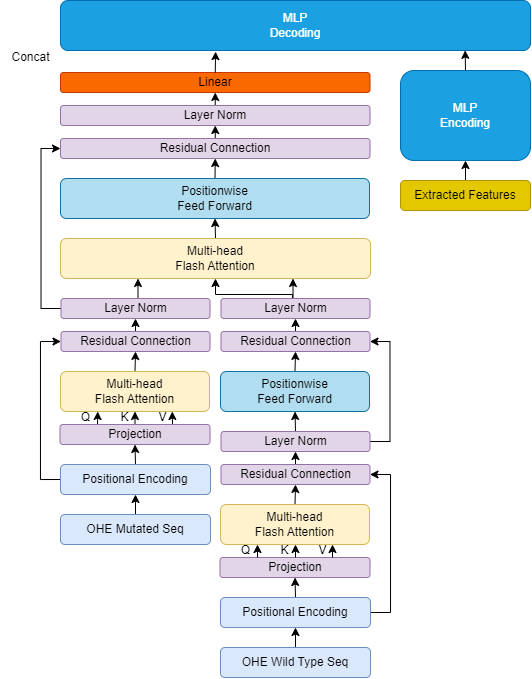
\includegraphics[width=0.8\textwidth]{transformer-architecture.png}
    \caption[Transformer Model Architecture]{Transformer Prime Editing Efficiency Prediction Model Architecture}
    \label{fig:transformer-model}
\end{figure}

\subsection{Architecture and Hyperparameter Tuning}

A number of architectural and hyperparameter choices were tested during the development of the transformer model.
The tuning of the model's architecture and hyperparameter was performed on the PRIDICT2.0 HEK293T for a balance between dataset size and training time.

Similar to PRIDICT, the size of the MLP layers were controlled using three parameters. The first is the mlp\_embed\_factor, which controls the size of the hidden layers in the MLP encoder and decoder. This is followed by the embed dimension of the MLP, which is the size of the output of the MLP embedder processing the feature vector. The last parameter is the number of encoder units inside of the MLP, where a encoder unit is a combination of two linear layers converting the data from embed dimension to embed dimension * mlp\_embed\_factor, followed by dropout and layer normalization.

To reduce the computational cost by testing many parameters at the same times and forming a large parameter grid, the tuning was conducted in two separate stages, with the first stage of tuning focusing on the a number of design decisions of the model architecture. To begin with, a number of alternative attention mechanisms were tested, using the scalar dot product attention as a baseline. 

% Describe flash transformer
To alleviate the quadratic computational cost of the scalar dot product attention model, flash attention was included as a more efficient alternative to the self-attention mechanism. 

Half precision was required by the flash attention to train and test the model. Half precision can significantly reduce memory usage and training time, achieving up to 8 times speed up when compared to single precision (float32)\cite{micikeviciusMixedPrecisionTraining2018}. However, certain small-magnitude gradients may fall out of range of half precision and become zero. This results in NaN values in the model's weights and losses, causing training to fail. As a result, the hugging face accelerator module was adopted to prevent the model from diverging during training. 

Additionally, global attention is not always necessary for lower level of the transformer model\cite{raeTransformersNeedDeep2020}, thus another 
possible improvement to the model is to use local attention for self-attention layers. The local attention only allows the model to attend to a fixed number of tokens within a certain window, reducing the computational cost of the attention mechanism and maybe improving the model's performance by focusing on the most relevant tokens.

However, during testing, neither the flash attention nor the local attention showed any significant improvement in the model's performance. Even with the hugging face's accelerator module, the mixed precision training still causes around 1 out of 20 training runs to fail due to NaN values in the model's weights and losses, especially in model configurations with poor performances. Additionally, no significant improvement in either training time or performance was observed when using flash attention when training on the network with 1 encoder and decoder layer using 2 attention heads (one head works on CG representation, the other works on AT representation, performance comparison with pearson's $r$ of 0.79 vs 0.79 across 5 repeated runs, $p>0.1$, paired t-test) compared to scalar product attention. On the same configuration of 1 encoder and 1 decoder, the local attention mechanism also did not show any significant improvement in the model's performance (pearson's $r$ of 0.78 vs 0.79 for with and without local attention respectively, $p>0.1$, paired t-test).

Additionally, although having previously established that the usage of embedding does not significantly improve the DeepPrime and PRIDICT models' performance, the influence of using PRIDICT's functional annotation still needs to be investigated. Using the same configuration with local attention enabled, again no significant improvement was observed in the model's performance (3 heads used for annotated representation, with 2 heads processing ATGC representation as before, and 1 extra head processing the PBS and RTT representation, pearson's $r$ of 0.79 vs 0.79, $p>0.1$, paired t-test).

As a result, the final model was configured with the scalar dot product attention mechanism with local attention used during the self-attention layers, without the usage of flash attention or functional annotation.

The next stage focuses on the parameter size of the model. Since the MLP modules were already optimized by Yu at al in their DeepPrime study, the size of the MLP layers were kept constant. The size of the transformer is mostly controlled by twi parameters: the number of encoder and decoder layers, and the mlp embedding size of the positional feedforward layers. Additionally, the dropout rate was also optimized in this stage as it determines the amount of information that is retained during training. A grid search was conducted on the PRIDICT2.0 HEK293T dataset, using the following configuration for each parameter:

\begin{itemize}[itemsep=-0mm]
    \item \textcolor{blue}{Number of Encoder/Decoder Layers}: 1, 2, 3
    \item \textcolor{blue}{Positional Feedforward Embedding Size}: 100, 150, 200
    \item \textcolor{blue}{Dropout Rate}: 0.1, 0.3, 0.5
\end{itemize}

The full list of performance of the models using each configuration can be found in \autoref{appendix:transformer-hyperparameter-tuning}. Overall, the best configuration for the transformer model was the simplest 1 encoder and 1 decoder layer with 2 attention heads, using a low dropout rate of 0.1. Stacking and increasing the number of hidden units in the positional feedforward layers significantly increased the model's training time and memory usage, while decreasing the overall performance (Pearson's $r$ of 0.78 vs 0.81, stacking with 3 encoder and decoder units while increasing the number of hidden units to 200 vs the base configuration with 1 encoder decoder unit and 100 hidden units), possibly due to overfitting.

\section{Development of pegRNA Design Web Tool}

To facilitate the use of the model in the community, a web tool was developed for users to input their target edit and receive the best pegRNA design as per the model's prediction. The web tool was implemented using the Django framework for easier interaction with Python scripts. 

User input should be in the PRIDICT format of \{at-lesat-100bp\}-(before-edit/after-edit)-\{at-lesat-100bp\}. The user response is then handled by the prediction API endpoint, which would parse the input into original and mutated sequence as well as edit location, type and length. A number of pegRNAs would then be proposed accordingly in the standard data format, which is then converted to the suitable formats for the models. The best performing model would then be used to predict the editing efficiency of the candidate pegRNAs. 


The result is returned as a JSON response and is parsed by the front end as a table of pegRNA candidates with their corresponding editing efficiency. The pegRNA's composition with regard to the wild type sequence can also be visualized by selecting a particular result for easier interpretation.

Other than the model itself, an algorithm for suggesting candidate pegRNAs given a desirable edit was also implemented. Supposing the nick is done at 3bp upstream of the PAM, for the edit to be possible, the PAM sequence must be at most 3bp downstream of the edit start location (in which case LHA length is 0). 

This requirement has the most significant constraint on the LHA length, as it always starts at the nick site 3bp upstream of the PAM and must be able to reach the edit location. PBS and RHA, on the other hand, are much more flexible in length, as they can be extended to their 3' and 5' ends respectively.
However, as discussed in \autoref{sec:determinants}, the length of LHA, RHA and PBS all have significant impact on the editing efficiency. To come up with a recommended range for these parameters, a more detailed analysis of the relationship between the lengths and the editing efficiency was conducted.

\begin{figure}
    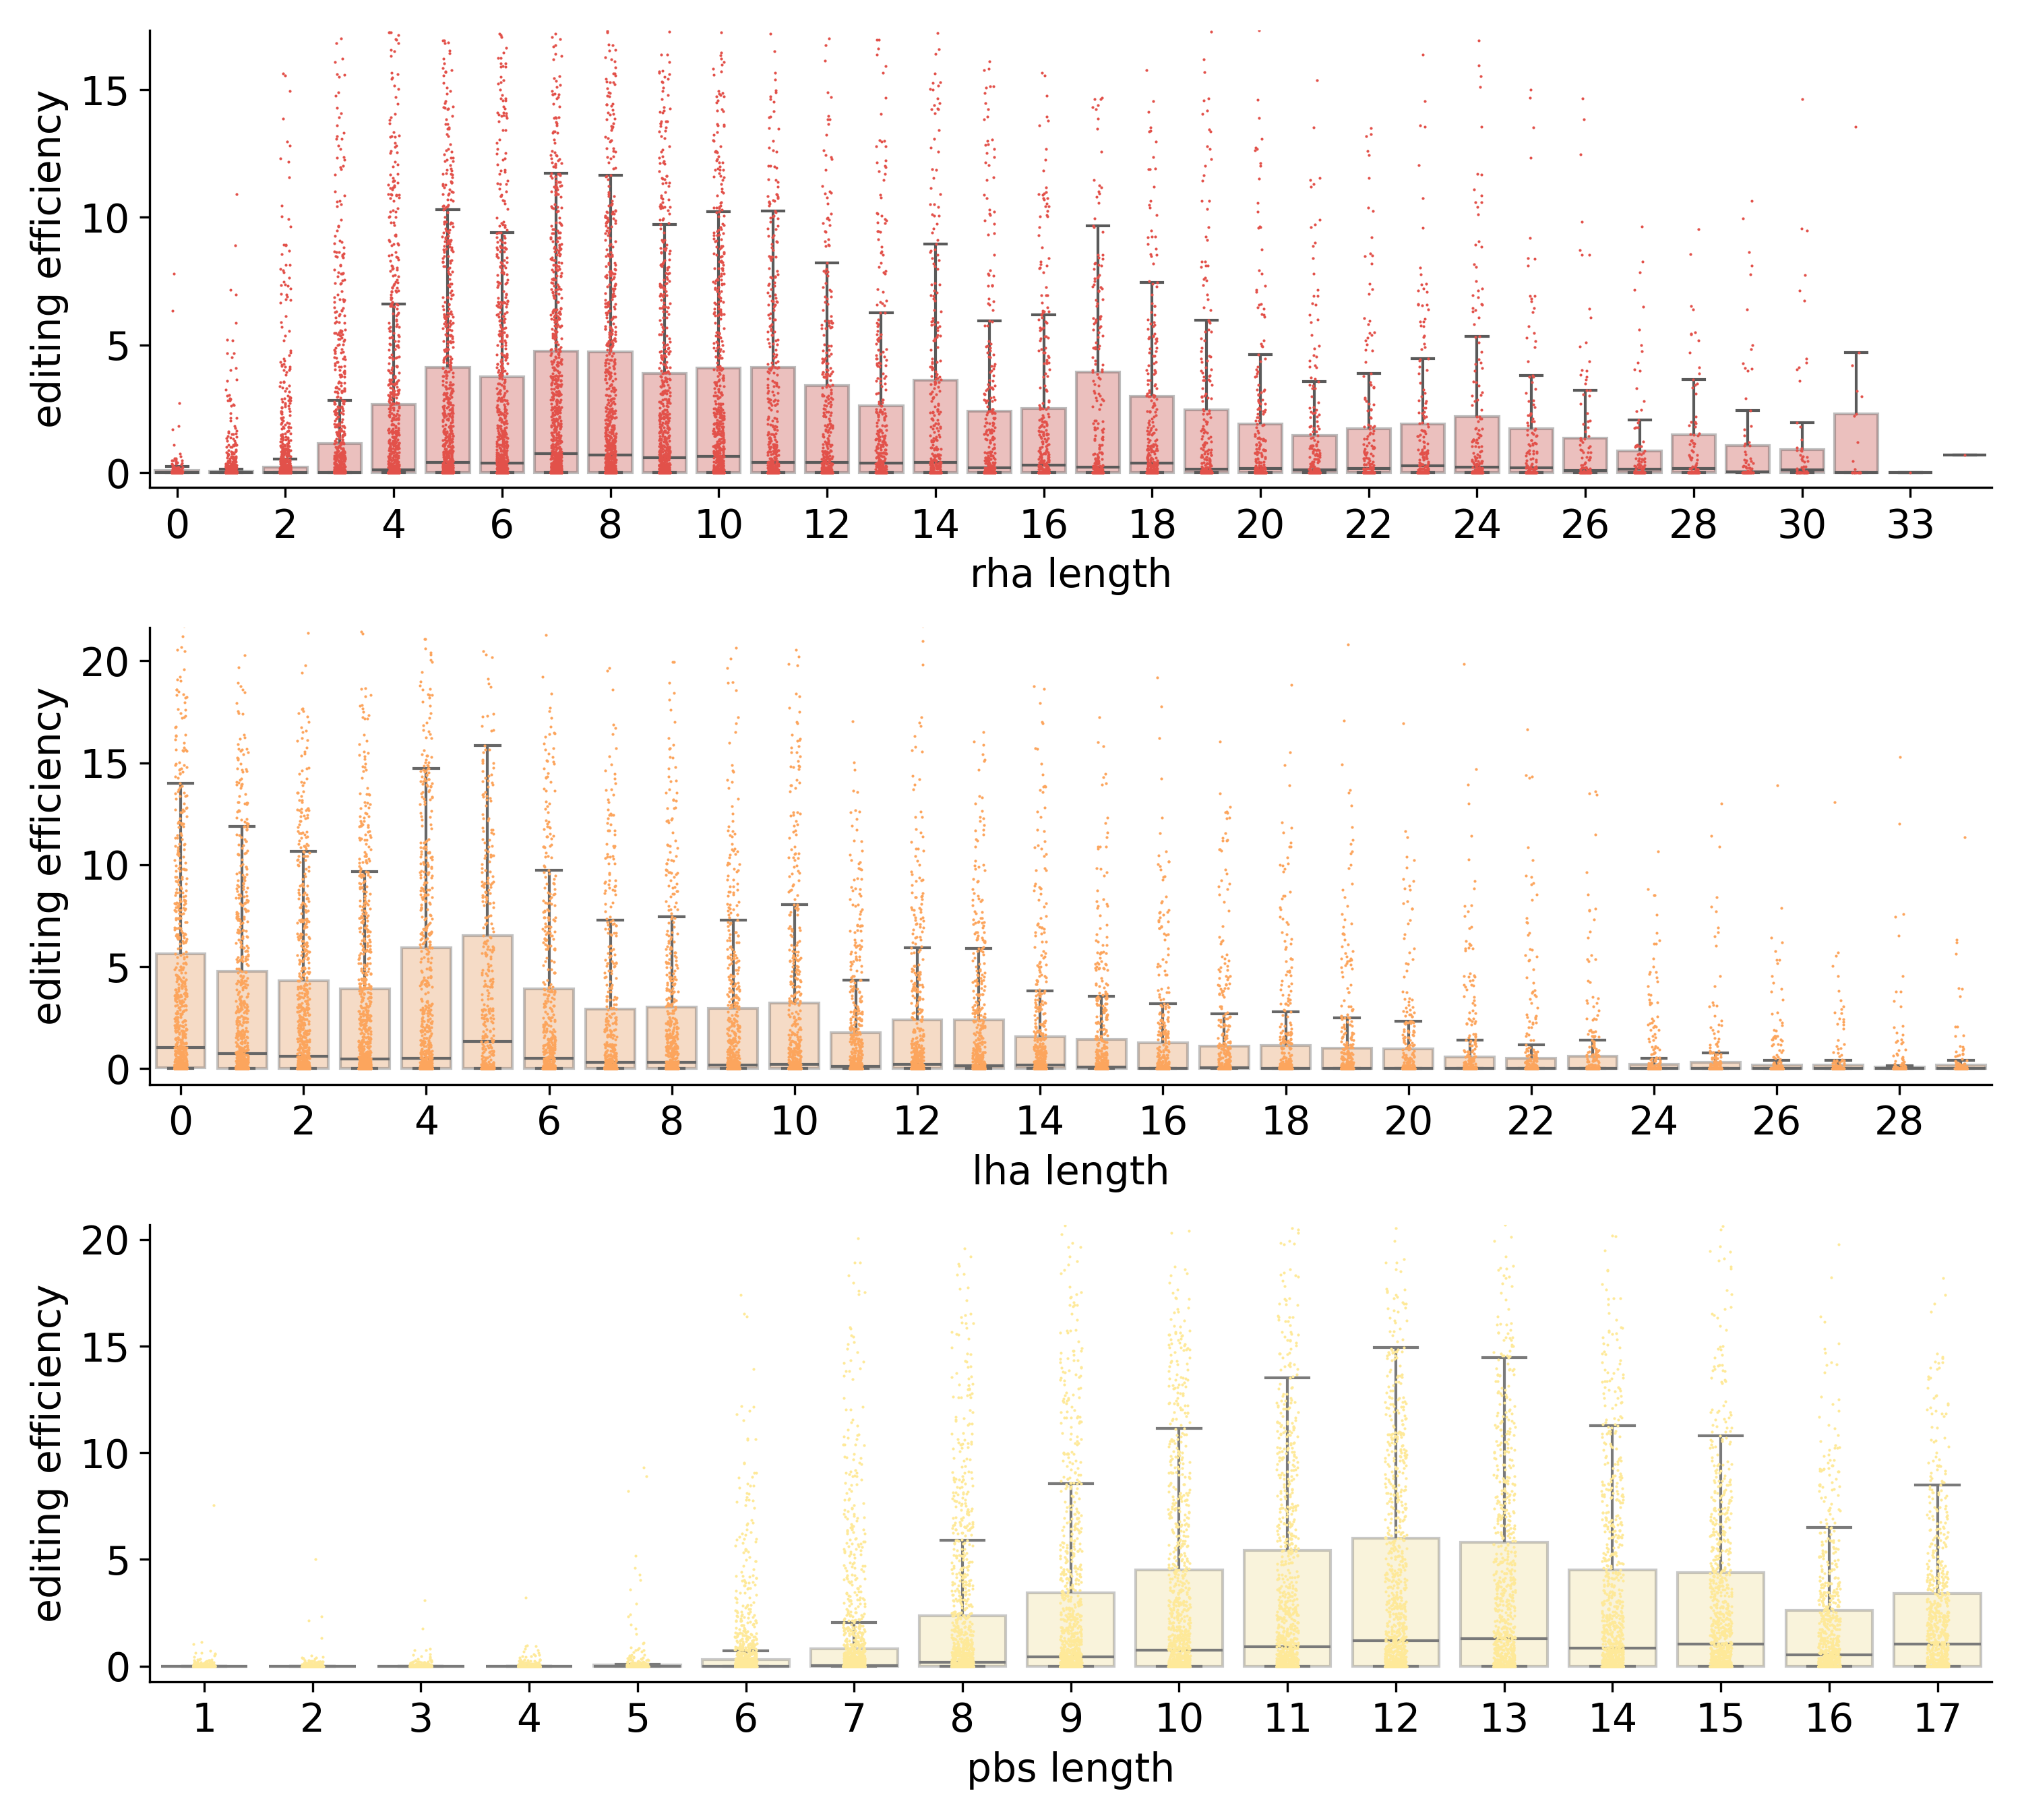
\includegraphics[width=\textwidth]{lha-rha-pbs-length-requirement.png}
    \caption[Relationship between LHA, RHA and PBS length and editing efficiency]{Relationship between PBS (top), RHA (middle) and LHA (bottom) length and editing efficiency. Data from all of the DeepPrime and PRIDICT datasets was used in the analysis for better generalizability. Random samples of 5\% of the individual data pointso were plotted as a strip plot on top of the box plot to shw real data while keeping the figure from clutering. Y axis is limited to a max value of 5 + 1.5 * IQR to further improve readability. }
    % The values associated with rha length over 30bp were omitted due to the small number of data points and very low efficiency.
    \label{fig:lha-rha-pbs-length}
\end{figure}


Shown in \autoref{fig:lha-rha-pbs-length}, the relationship between the lengths of LHA, RHA and PBS and the editing efficiency was analyzed using the all data in the DeepPime and PRIDICT datasets. Consistent with Yu et al, 2023's finding, editing editing efficiency plateaued with RHA length of 7-12bp. Since RHA is the component with the greatest flexibility in length as it does not depend on target location, I decided to only use the 7-12bp range where the corresponding efficiency is the highest so that the resulting search space can be smaller.  As for LHA, the efficiency was shown to decrease with longer LHA length, with an elbow point at around 13bp, where the decrease in performance with regard to the lha length speeded up. Thus, the recommended distance between the nick and the edit location is set to 0-13bp, and this is only extended if no suitable PAM is found within the range. Last but not least, as expected, PBS length's impact on the editing efficiency is roughly normally distributed, with the highest efficiency at around 12bp. Decent performance can be observed from 8bp all the way up to the highest recorded value of 17bp, which covers the entire range of the protospacer upstream of the nick site. Thus, although the SHAP analysis showed that long PBS can be detrimental to the editing efficiency, the range of PBS length was still set to 8-17bp.

In summary, unless specified otherwise by the users, the algorithm would only propose pegRNAs with component length in the range specified in \autoref{tab:recommended-range}. The recommending range would result in a maximum of 585 pegRNAs (true number is usually much smaller as LHA location is heavily constrained), which would then be processed and evaluated by the model to produce the estimated editing efficiency.

\begin{table}[h]
    \centering
    \begin{tabular}{c|c|c}
        % \hline
        \textbf{Component} & \textbf{Min Length} & \textbf{Max Length} \\
        \hline
        LHA & 0 & 13 \\
        RHA & 7 & 12 \\
        PBS & 8 & 17 \\
        % \hline
    \end{tabular}
    \caption{Recommended range for LHA, RHA and PBS length}
    \label{tab:recommended-range}
\end{table}


Limited by the scale and funding of this project, the web tool was not deployed to a public server, but instead packaged in a container for local use with Docker. 

It is also accessible using Python with Django and Pytorch installed by executing:

\verb|python webtool/manage.py runserver|

suppose that the user is in the root directory of the project. The web tool can then be accessed by visiting \verb|http://127.0.0.1:8000/|.